\documentclass[12pt]{article}
% header.tex

% page layout
%\usepackage[left=1in,right=1in,top=1in,footskip=25pt]{geometry} 
\usepackage{setspace}
%\doublespacing
\onehalfspacing
% \usepackage{changepage}

% define math norms
\usepackage{amsmath,amsthm,amssymb,amsfonts}
\usepackage{mathtools}
%\DeclarePairedDelimiter\norm\lVert\rVert

%% define a rotated tilted `less & greater than' with certain rotated angles
\usepackage{amssymb,stackengine,graphicx,scalerel}
\newcommand\rotlesssim{\mathrel{\ensurestackMath{\ThisStyle{%
  \stackengine{-.4\LMex}{\SavedStyle<}{%
    \rotatebox{-15}{$\SavedStyle\sim$}}{U}{r}{F}{T}{S}}}}}
\newcommand\rotgtrsim{\mathrel{\ensurestackMath{\ThisStyle{%
  \stackengine{-.4\LMex}{\SavedStyle>}{%
    \rotatebox{15}{$\SavedStyle\sim$}}{U}{l}{F}{T}{S}}}}}

% notations
\usepackage{etoolbox}
\usepackage{datagidx}

% lists
\usepackage{enumitem}
% Load dsfont this to get proper indicator function (bold 1) with \mathds{1}:
\usepackage{dsfont}
\usepackage{centernot}

% graphics
\usepackage{graphicx}
\DeclareGraphicsExtensions{.pdf,.png,.jpg}
\graphicspath{ {fig/} }
\usepackage{wrapfig}
\usepackage{graphics}

% tables
\usepackage{multirow}
\usepackage{float}
\setlength{\footskip}{40pt}
\font\myfont=cmr12 at 20pt

% theory
\newtheorem{lemma}{Lemma}
\newtheorem{theorem}{Theorem}

% algorithms
\usepackage{algorithm2e}%[linesnumbered,ruled,vlined]

% table of contents
\usepackage[utf8]{inputenc}
%\usepackage{blindtext}

% others: appendix, color and more
\usepackage[usenames,dvipsnames]{xcolor}
\usepackage{appendix}
\usepackage{titlesec}
%\usepackage{fancyhdr}
%\pagestyle{fancy}
%\setlength{\headheight}{14.5pt}
\usepackage{caption}

% references
\usepackage[authoryear,round,sort&compress]{natbib}%,round,compress,elide,comma
\bibliographystyle{plainnat}
%\usepackage[american]{babel}


% hyperref should come at the bottom
% Set up hyperlinks:
\definecolor{RefColor}{rgb}{0,0,.65}
\usepackage[colorlinks,linkcolor=RefColor,citecolor=RefColor,urlcolor=RefColor]{hyperref} %hidelinks
\renewcommand{\eqref}[1]{Equation~(\ref{#1})}
\renewcommand{\chapterautorefname}{Chapter}
\renewcommand{\sectionautorefname}{Section}

%\usepackage[capitalize]{cleveref}
%\crefname{appsec}{appendix}{appendices}
%\Crefname{appsec}{Appendix}{Appendices}



% defs.tex
% define custom notation, commands, etc.

%%%%%%%%%%%%%%%%%%%%%%%%%%%%%%%%%%%%%%%%%%%%%%%%%%%%%%%%%%
%% full alphabets of different styles 
% bf series
\def\bfA{\mathbf{A}}
\def\bfB{\mathbf{B}}
\def\bfC{\mathbf{C}}
\def\bfD{\mathbf{D}}
\def\bfE{\mathbf{E}}
\def\bfF{\mathbf{F}}
\def\bfG{\mathbf{G}}
\def\bfH{\mathbf{H}}
\def\bfI{\mathbf{I}}
\def\bfJ{\mathbf{J}}
\def\bfK{\mathbf{K}}
\def\bfL{\mathbf{L}}
\def\bfM{\mathbf{M}}
\def\bfN{\mathbf{N}}
\def\bfO{\mathbf{O}}
\def\bfP{\mathbf{P}}
\def\bfQ{\mathbf{Q}}
\def\bfR{\mathbf{R}}
\def\bfS{\mathbf{S}}
\def\bfT{\mathbf{T}}
\def\bfU{\mathbf{U}}
\def\bfV{\mathbf{V}}
\def\bfW{\mathbf{W}}
\def\bfX{\mathbf{X}}
\def\bfY{\mathbf{Y}}
\def\bfZ{\mathbf{Z}}

% bb series
\def\bbA{\mathbb{A}}
\def\bbB{\mathbb{B}}
\def\bbC{\mathbb{C}}
\def\bbD{\mathbb{D}}
\def\bbE{\mathbb{E}}
\def\bbF{\mathbb{F}}
\def\bbG{\mathbb{G}}
\def\bbH{\mathbb{H}}
\def\bbI{\mathbb{I}}
\def\bbJ{\mathbb{J}}
\def\bbK{\mathbb{K}}
\def\bbL{\mathbb{L}}
\def\bbM{\mathbb{M}}
\def\bbN{\mathbb{N}}
\def\bbO{\mathbb{O}}
\def\bbP{\mathbb{P}}
\def\bbQ{\mathbb{Q}}
\def\bbR{\mathbb{R}}
\def\bbS{\mathbb{S}}
\def\bbT{\mathbb{T}}
\def\bbU{\mathbb{U}}
\def\bbV{\mathbb{V}}
\def\bbW{\mathbb{W}}
\def\bbX{\mathbb{X}}
\def\bbY{\mathbb{Y}}
\def\bbZ{\mathbb{Z}}

% cal series
\def\calA{\mathcal{A}}
\def\calB{\mathcal{B}}
\def\calC{\mathcal{C}}
\def\calD{\mathcal{D}}
\def\calE{\mathcal{E}}
\def\calF{\mathcal{F}}
\def\calG{\mathcal{G}}
\def\calH{\mathcal{H}}
\def\calI{\mathcal{I}}
\def\calJ{\mathcal{J}}
\def\calK{\mathcal{K}}
\def\calL{\mathcal{L}}
\def\calM{\mathcal{M}}
\def\calN{\mathcal{N}}
\def\calO{\mathcal{O}}
\def\calP{\mathcal{P}}
\def\calQ{\mathcal{Q}}
\def\calR{\mathcal{R}}
\def\calS{\mathcal{S}}
\def\calT{\mathcal{T}}
\def\calU{\mathcal{U}}
\def\calV{\mathcal{V}}
\def\calW{\mathcal{W}}
\def\calX{\mathcal{X}}
\def\calY{\mathcal{Y}}
\def\calZ{\mathcal{Z}}
%%%%%%%%%%%%%%%%%%%%%%%%%%%%%%%%%%%%%%%%%%%%%%%%%%%%%%%%%%

%%%%%%%%%%%%%%%%%%%%%%%%%%%%%%%%%%%%%%%%%%%%%%%%%%%%%%%%%%
% quasi-universal probabilistic and mathematical notation
% my preferences (modulo publication conventions, and clashes like random vectors):
%   vectors: bold, lowercase
%   matrices: bold, uppercase
%   operators: blackboard (e.g., \mathbb{E}), uppercase
%   sets, spaces: calligraphic, uppercase
%   random variables: normal font, uppercase
%   deterministic quantities: normal font, lowercase

\newcommand{\R}{\texttt{R}\ }
\newcommand{\cpp}{\texttt{C++}\ }

% lists
\makeatletter
\newcommand{\blist}[1]{\begin{enumerate}[label=\roman*.]\label{list:#1}}
\newcommand{\elist}{\end{enumerate}}
\makeatother

% equations
\makeatletter
\newcommand{\beq}[1]{\begin{equation}\label{eq:#1}}
\newcommand{\eeq}{\end{equation}}
\makeatother

\newcommand{\fr}[1]{\frac{1}{#1}}
\newcommand{\lr}[1]{\left(#1\right)}
\newcommand{\norm}[1]{\left\lVert #1 \right\rVert}
\newcommand{\abs}[1]{\left\lvert #1 \right\rvert}

\DeclareMathOperator*{\Lambert}{\mathrm{Lambert}_0}
\DeclareMathOperator*{\diag}{diag}
\DeclareMathOperator*{\argmin}{argmin}
\newcommand{\Argmin}[1]{\underset{#1}{\argmin\ }}
\def\sumN{\sum_{i=1}^n}

% binary relations
\def\condind{{\perp\!\!\!\perp}} %independence/conditional independence
\def\equdist{\stackrel{\text{\rm\tiny d}}{=}} %equal in distribution
\def\equas{\stackrel{\text{\rm\tiny a.s.}}{=}} %equal almost surely
\def\simiid{\sim_{\mbox{\tiny iid}}} %sampled i.i.d

% common vectors and matrices
\def\onevec{\mathbf{1}}
\def\iden{\mathbf{I}} % identity matrix
\def\supp{\text{\rm supp}}

\def\gDeltakk{\Delta^{(k+1)}}
\def\gDeltakkX{\Delta^{(x,k+1)}}
\def\gDeltak{\Delta^{(k)}}
\def\gDeltakX{\Delta^{(x,k)}}
\def\gDelta{\Delta^{(1)}}
\def\gDeltaX{\Delta^{(x,1)}}
\def\gDkk{D^{(k+1)}}
\def\gDk{D^{(k)}}
\def\gD1{D^{(1)}}
\def\Dxk{D^{(x,k)}}
\def\Dxkk{D^{(x,k+1)}}
\def\tDxk{\tilde{D}^{(x,k+1)}}

% misc
% floor and ceiling
\DeclarePairedDelimiter{\ceilpair}{\lceil}{\rceil}
\DeclarePairedDelimiter{\floor}{\lfloor}{\rfloor}
\newcommand{\argdot}{{\,\vcenter{\hbox{\tiny$\bullet$}}\,}} %generic argument dot
%%%%%%%%%%%%%%%%%%%%%%%%%%%%%%%%%%%%%%%%%%%%%%%%%%%%%%%%%%

%%%%%%%%%%%%%%%%%%%%%%%%%%%%%%%%%%%%%%%%%%%%%%%%%%%%%%%%%%
% Notations 

% Define a database of notations
\newgidx{notation}{Notation}
% Set this as the default database so we don't have to keep
% explicitly mentioning it
\DTLgidxSetDefaultDB{notation}

% Define some terms
\newterm[description={description for A}]{\gDeltakk}

% Fake a counter called "notation" to be used in the location list
% Two digits are used to make the substring comparison easier
% (used in the condition of \printterms)
%\makeatletter
%\newcommand*{\twodigits}[1]{\two@digits{\value{#1}}}
%\newcommand*{\thenotation}{C\twodigits{chapter}.\thepage}
%\makeatother


% Define a command to print the notation list
\newcommand{\printnotation}{
    \bgroup
    \edef\locationprefix{}
    \printterms
     [heading={\section*}, % put the heading in an unnumbered section    
     condition={\DTLisSubString{\Location}{\locationprefix}},
     sort={}, % suppress sorting - do it manually    
     location=first, % only show first location    
     columns=1 % one column list - change as required   
     ]%
    \egroup
    % Add a vertical gap so it's not right on top of the next paragraph
    \vskip\baselineskip
    % Set the after heading flag (remove if not required):
    \csuse{@afterheading}
    % Something is confusing the rerun warnings, so disable it and 
    % just remember to use multiple LaTeX runs: 
    \csdef{@datagidx@dorerun@warn}{}%
}

% Patch \datagidx@formatlocation so that it strips the location prefix
% and inserts "p." before the location
\makeatletter
\let\orgformatlocation\datagidx@formatlocation
\renewcommand*{\datagidx@formatlocation}[2]{%
  \expandafter\DTLsplitstring\expandafter{#2}{.}{\locprefix}{\locsuffix}%
  \orgformatlocation{#1}{p.\locsuffix}%
}
\makeatother

% after all terms have been defined, so manually to avoid the
% redundancy of sorting each time the notation list is display.
\dtlsort{Sort}{notation}{\dtlwordindexcompare}


%\usepackage{arxiv}

\usepackage[utf8]{inputenc} % allow utf-8 input
\usepackage[T1]{fontenc}    % use 8-bit T1 fonts
\usepackage{url}            % simple URL typesetting
\usepackage{booktabs}       % professional-quality tables
\usepackage{amsfonts}       % blackboard math symbols
\usepackage{nicefrac}       % compact symbols for 1/2, etc.
\usepackage{microtype}      % microtypography
\usepackage{lipsum}
% \usepackage{graphicx}
\graphicspath{ {./images/} }
\usepackage[margin=2.5cm,nohead]{geometry}
\usepackage{authblk}
\newcommand{\email}[1]{\href{mailto:#1}{#1}}

\title{RtEstim: Effective reproduction number estimation with trend filtering}

\author[a,1]{Jiaping Liu}
\author[b]{Zhenglun Cai}
\author[a]{Paul Gustafson}
\author[a]{Daniel J. McDonald}

\affil[a]{Department of Statistics, The University of British Columbia}
\affil[b]{Centre for Health Evaluation and Outcome Sciences, The University of
British Columbia}

\begin{document}

\maketitle

\begin{abstract}
  To understand the transmissibility and spread of infectious diseases,
  epidemiologists turn to estimates of the effective reproduction number.
  While many approaches exist, their utility may be limited by the
  challenges of surveillance data collection. Arbitrary model assumptions
  that are unverifiable with data alone and sophisticated, though
  computationally inefficient, frameworks that
  are critical limitations for many
  existing approaches. We propose a Poisson trend filtering estimator
  \RtEstim\ for effective reproduction numbers estimation. \RtEstim\
  produces remains accurate even under some process misspecifications and
  is computationally efficient,
  even for large-scale data. The 
  implementation is easily accessible in a lightweight \texttt{R} package
  \href{https://dajmcdon.github.io/rtestim/index.html}{\texttt{rtestim}}.

  {\bf Keywords:} \attn{1--2 word phrases $|$ that aren't in the title.}
\end{abstract}

\footnotetext[1]{To whom correspondence should be
  addressed. E-mail: \email{jiaping.liu@stat.ubc.ca}} 
% Technical summary including research objective, method, results, and conclusions.

%\thispagestyle{empty}
%\pagenumbering{roman}
%\setcounter{page}{1}

%\printnotation
%\input{doc/notations.tex}
\newpage
%\hypersetup{linkcolor=black}
\tableofcontents % for easy edits, remove later

%\listoffigures

\clearpage
%\pagenumbering{arabic}
%\setcounter{page}{1}

% research proposal
\section{Introduction}
\label{sec:intro}

The effective reproduction number is defined to be the average number of
secondary infections caused by a primary infection that occurred sometime in the past. 
Also called the instantaneous reproduction number, it is a key quantity
for understanding infectious disease dynamics including the potential size of an
outbreak and the required stringency of control measures.  Tracking the time
series of this quantity is useful for understanding whether or not
future infections are likely to increase or decrease from the current state. Let
$\calR(t)$ denote the effective reproduction number at time $t$. Practically, as
long as $\calR(t) < 1$, infections will decline gradually, eventually resulting
in a disease-free equilibrium, whereas when $\calR(t) > 1$, infections will
continue to increase, resulting in endemic equilibrium. While $\calR(t)$ is
fundamentally a continuous time quantity, it can be related to data only at
discrete points in time $t = 1,\ldots,n$. This sequence of effective
reproduction numbers over time is not observable, but, nonetheless, is easily
interpretable and retrospectively describes the course of an epidemic.
Therefore, a number of procedures exist to estimate $\calR_t$ from different
types of observed incidence data such as cases, deaths, or hospitalizations,
while relying on various domain-specific assumptions. Importantly, accurate
estimation of effective reproduction numbers relies heavily on the quality of
the available data, and, due to the limitations of data collection, such as
underreporting and lack of standardization, estimation methodologies rely on
various assumptions to compensate. Because model assumptions may not be easily
verifiable from data alone, it is also critical for any estimation procedure to
be robust to model misspecification. 


Many existing approaches for effective reproduction number estimation are
Bayesian: they estimate the posterior distribution of $\calR_t$ conditional on
the observations. One of the first such approaches is the software \EpiEstim\
\citep{cori2020package}, described in \cite{cori2013new}. This method is
prospective, in that it uses only observations available up to time $t$ in order
to estimate $\calR_t$ for each $i = 1,\ldots, t$. An advantage of \EpiEstim\ is
its straightforward statistical model: new incidence data follows the Poisson
distribution conditional on past incidence combined with the conjugate gamma
prior distribution for $\calR_t$ with fixed hyperparameters. Additionally, the
serial interval distribution, the distribution of the period between onsets of
primary and secondary infections in a population, is fixed and known. For this
reason, \EpiEstim\ requires little domain expertise for use, and it is
computationally fast. \cite{thompson2019improved} modified this method to
distinguish imported cases from local transmission and simultaneously estimate
the serial interval distribution. \cite{nash2023estimating} further extended
\EpiEstim\ by using ``reconstructed'' daily incidence data to handle irregularly
spaced observations. Recently, \cite{abbott2020estimating} proposed a Bayesian
latent variable framework, \texttt{EpiNow2} \citep{EpiNow2}, which leverages
incident cases, deaths or other available streams simultaneously along with
allowing additional delay distributions (incubation period and onset to
reporting delays) in modelling.  
\cite{lison2023generative} proposed an extension that handles missing data by
imputation followed by a truncation adjustment. These modifications are intended
to increase accuracy at the most recent (but most uncertain) timepoints, to aid 
policymakers. \cite{parag2021improved} also proposed a Bayesian approach, 
\texttt{EpiFilter} based on the (discretized) Kalman filter and smoother. 
\texttt{EpiFilter} also estimates the posterior of $\calR_t$ given a Gamma 
prior and Poisson distributed incident cases. Compared to \EpiEstim, 
however, \texttt{EpiFilter} estimates $\calR_t$ retrospectively using all 
available incidence data both before and after time $t$, with the goal of being 
more robust in low-incidence periods. \cite{gressani2022epilps} proposed a 
Bayesian P-splines approach, \EpiLPS, that assumes negative Binomial distributed 
observations. \cite{trevisin2023spatially} also proposed a Bayesian model estimated 
with particle filtering to incorporate spatial structures. 
Bayesian approaches estimate the posterior distribution of the effective
reproduction numbers and possess the advantage that credible intervals may be
easily computed. A limitation of many Bayesian approaches, however, is that they
usually require more intensive computational routines, especially when observed
data sequences are long or hierarchical structures are complex.  Below, we
compare our method to two of the more computationally efficient Bayesian models,
\EpiEstim\ and \EpiLPS. 


There are also frequentist approaches for $\calR_t$ estimation.
\cite{abry2020spatial} proposed regularizing the smoothness of $\calR_t$ through
penalized regression with second-order temporal regularization, additional
spatial penalties, and with Poisson loss. \cite{pascal2022nonsmooth} extended
this procedure by introducing another penalty on outliers.
\cite{pircalabelu2023spline} proposed a spline-based model relying on the
assumption of exponential-family distributed incidence. \cite{ho2023accounting}
estimates $\calR_t$ while monitoring the time-varying level of overdispersion.
There are other spline-based approaches such as
\cite{azmon2014estimation,gressani2021approximate}, autoregressive models with
random effects \citep{jin2023epimix} that are robust to low incidence, and
generalized autoregressive moving average (GARMA) models
\citep{hettinger2023estimating} that are robust to measurement errors in
incidence data. 


%%%%%%%%%%%%%%%%%%%%%%%%%%%%%%% our approach %%%%%%%%%%%%%%%%%%%%%%%%%%%%%%%%
We propose a retrospective effective reproduction number estimator
called \RtEstim\ that requires only incidence data. Our model makes the
conditional Poisson assumption, similar to much of the prior work described
above, but is empirically more robust to misspecification. This estimator is 
defined by a convex optimization problem with Poisson loss and $\ell_1$ penalty 
on the temporal evolution of $\log(\calR_t)$ to impose smoothness over time. 
As a result, \RtEstim\ generates discrete splines, and the estimated curves (in
logarithmic space) appear to be piecewise polynomials of an order selected by the
user. Importantly, the estimates are locally adaptive, meaning that different
time ranges may possess heterogeneous smoothness. Because we penalize the
logarithm of $\calR_t$, we naturally accommodate the positivity requirement, in
contrast to related methods, can
handle large or small incidence measurements, and are automatically (reasonably)
robust to outliers without additional constraints. A small illustration using
three years of Covid-19 case data in Canada is shown in \autoref{fig:intro-fig} 
\citep{CovidTimelineCanada}.

\begin{figure}[!h]
  \centering
  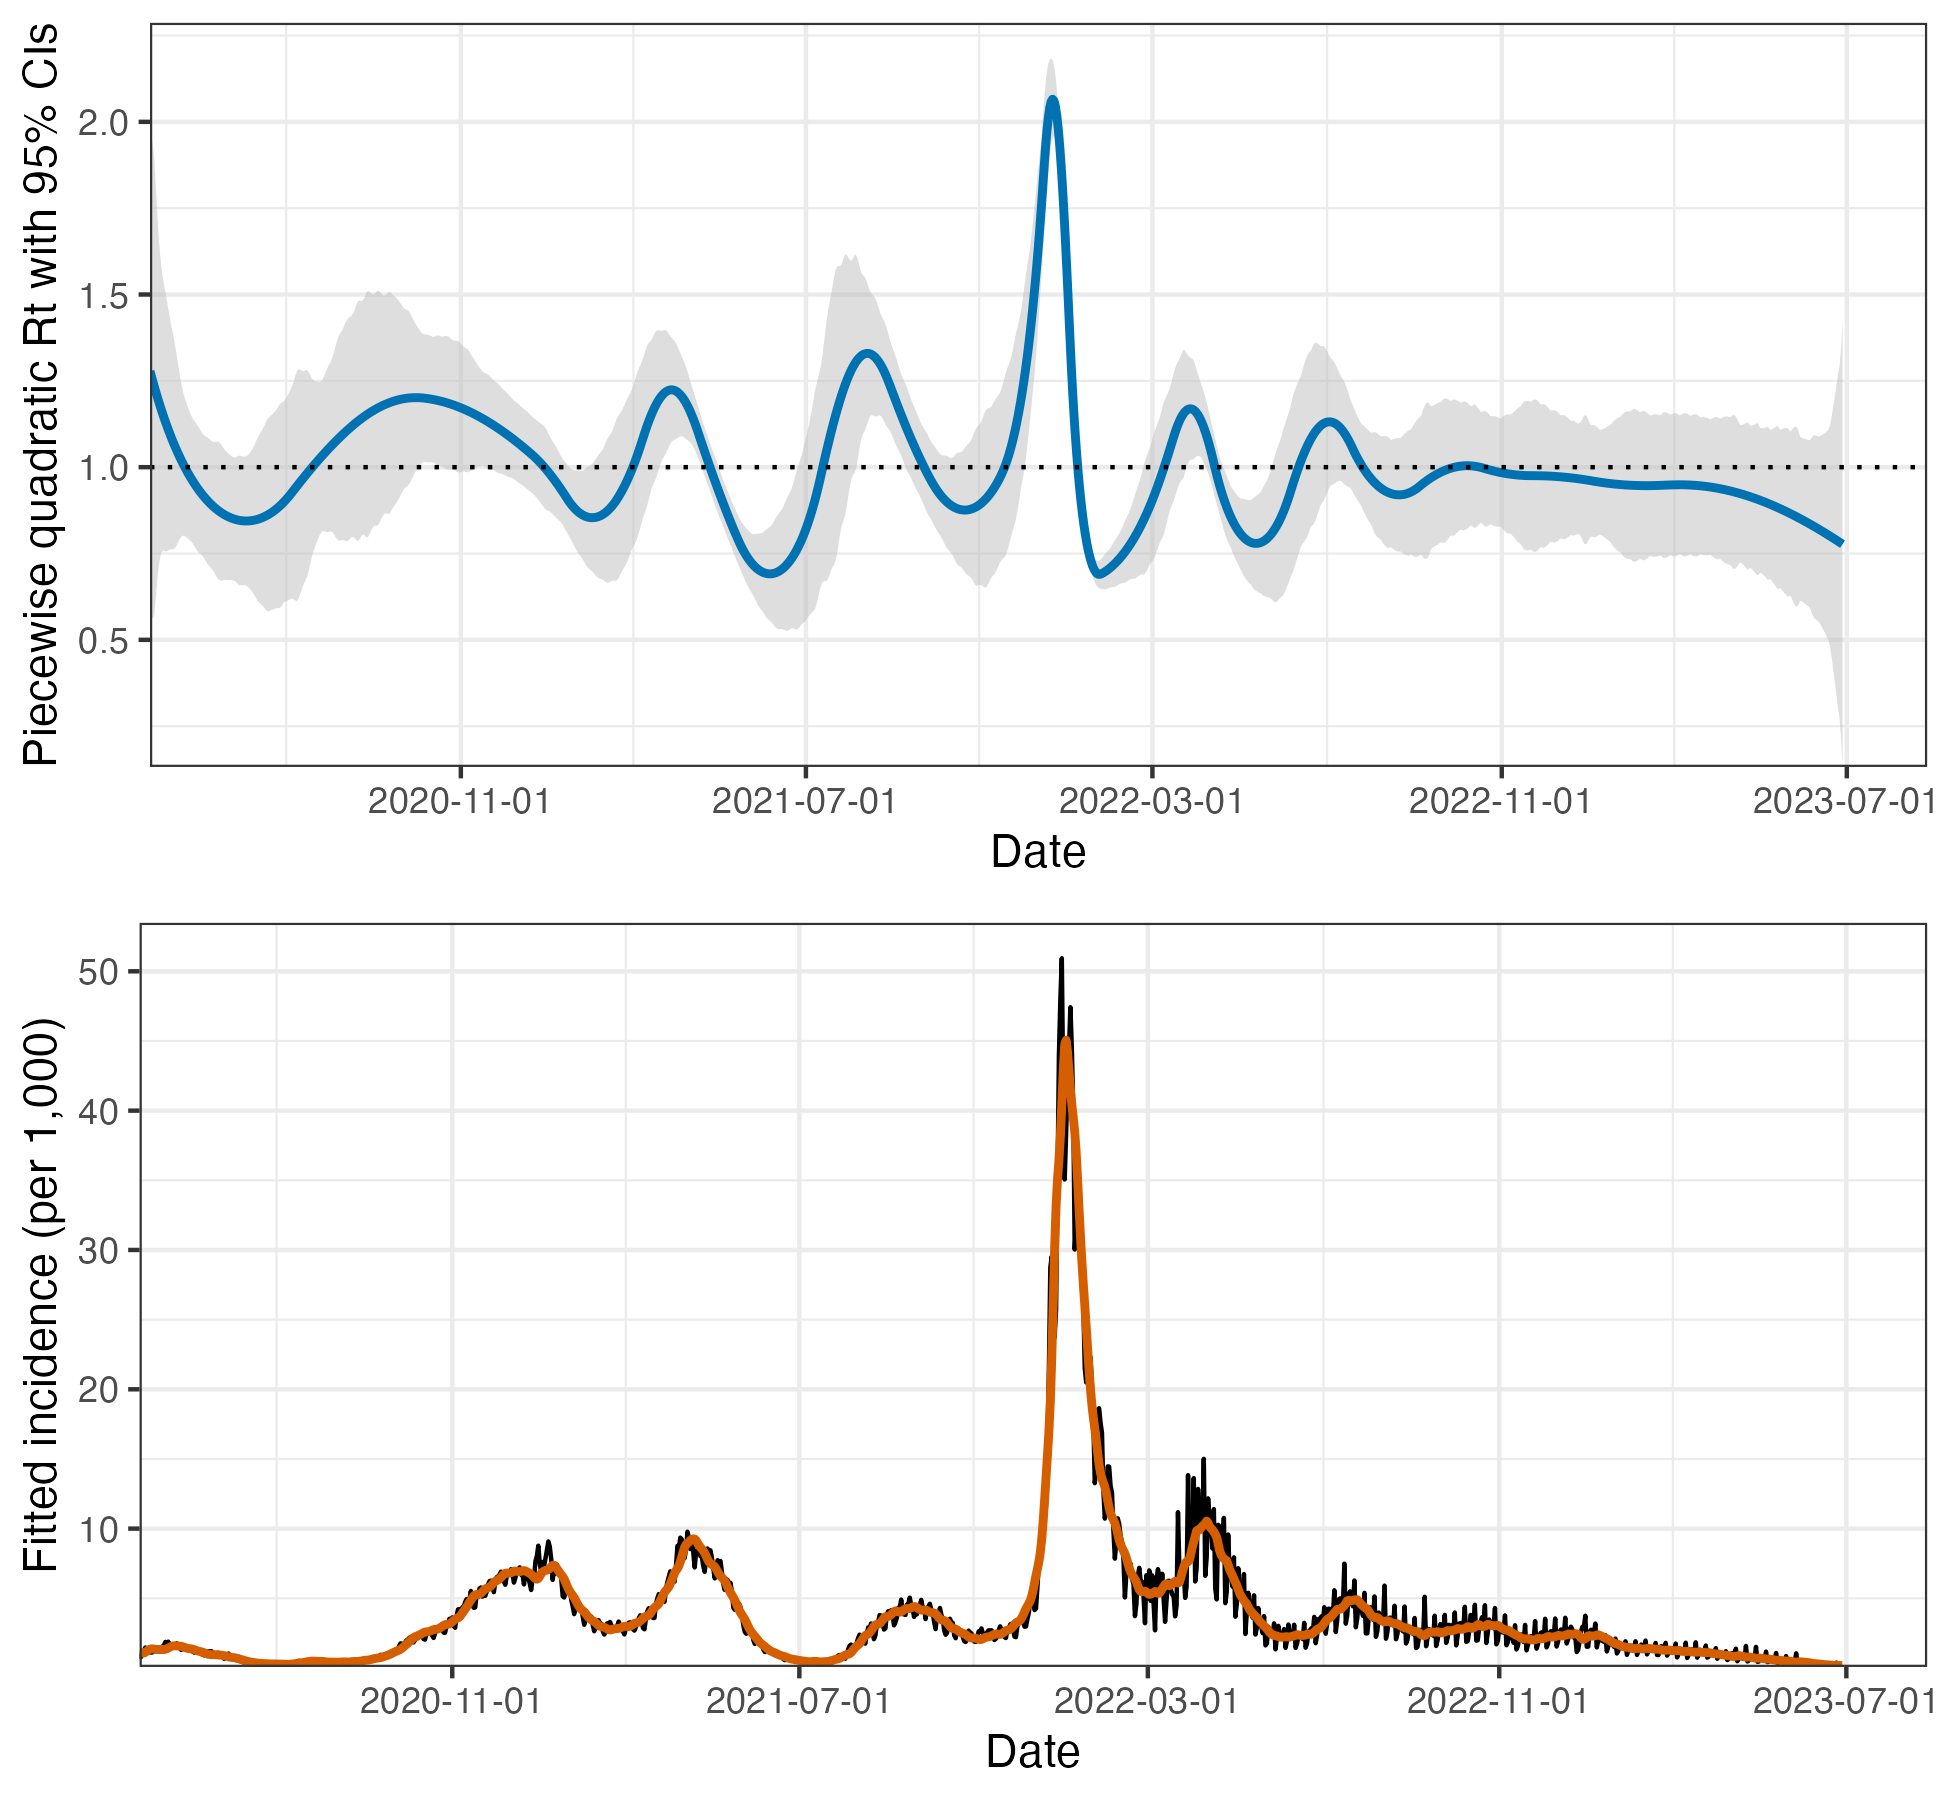
\includegraphics[width=.9\textwidth]{fig/intro-fig-new.png}
  \caption{A demonstration of effective reproduction number estimation 
  by \RtEstim\ and the corresponding predicted incident cases for the Covid-19 epidemic 
  in Canada during the period from March 28, 2020 to June 28, 2023. 
  In the top panel, the blue curve is the estimated piecewise
  quadratic $\calR_t$ and the gray ribbon is the corresponding 95\% confidence band. 
  The black curve in the bottom panel is the observed Covid-19 daily confirmed 
  cases, and the orange curve is the predicted incident cases
  corresponding to the estimated $\calR_t$.}
  \label{fig:intro-fig}
\end{figure}

While our approach is straightforward and requires little domain knowledge for
implementation, we also implement a number of refinements. 
We use a proximal Newton method to solve the convex optimization problem along
with warm starts to produce estimates efficiently, typically in a matter of 
seconds, even for long sequences of data. In a number of simulation experiments, 
we show empirically that our approach is more accurate than existing methods at 
estimating the true effective reproduction numbers. 


The manuscript proceeds as follows. We first introduce the methodology of
\RtEstim\ including the renewal equation and the development of Poisson
trend filtering estimator. We explain how this method could be interpreted from
the Bayesian perspective, connecting it to previous work in this context. We
provide illustrative experiments comparing our estimator to \EpiEstim\ and
\EpiLPS. We then apply our \RtEstim\ on the Covid-19 pandemic incidence in
British Columbia and the 1918 influenza pandemic incidence in the United States. 
Finally, we conclude with a discussion of the advantages and limitations of our 
approach and describe practical considerations for effective reproduction number
estimation.
  
\section{Methods}

\subsection{Renewal model for incidence data} 

The effective reproduction number $\calR(t)$ is defined to be the expected
number of secondary infections at time $t$ produced by a primary infection
sometime in the past. To make this precise, denote the number of new infections
at time $t$ as $y(t)$. Then the total primary infectiousness can be written as
$\eta(t) := \int_0^{\infty} p(i) y(t-i) \diff i$, where $p(i)$ is the
probability that a new secondary infection is the result of a primary infection
that occurred $i$ time units in the past. The effective reproduction number is then given
as the value that equates
\begin{equation} \label{eq:pre-renew-equation}
  \bbE[y(t) \mid y(j),\ j<t]=\calR(t)\eta(t)=\calR(t)\int_0^\infty p(i)y(t-i)\diff i,
\end{equation}
otherwise known as the renewal equation. The period between primary and secondary
infections is exactly the generation time of the disease, but given real data,
observed at discrete times (say, daily) this delay distribution must be discretized
into contiguous time intervals,
say, $(0,1], (1,2], \dots$, which results in the sequence $\{p_i\}_0^\infty$
corresponding to observations $y_t$ and resulting in the
discretized version of \eqref{eq:pre-renew-equation},
\begin{equation} \label{eq:renew-equation}
  \bbE[y_t \mid y_1,\ldots,y_{t-1}]=\calR_t\eta_t=\calR_t\sum_{i = 1}^\infty p_i y_{t-i}.
\end{equation}
Many approaches to estimating $\calR_t$ rely on \eqref{eq:renew-equation} as
motivation for their procedures, among them, \EpiEstim\ \citep{cori2013new} 
and \texttt{EpiFilter} \citep{parag2021improved}. 


In most cases, it is safe to assume that infectiousness disappears beyond 
$\tau$ timepoints ($p(i) = 0$ for $i > \tau$), resulting in the truncated integral 
of the generation interval distribution $\int_0^\tau p(i)\diff i = 1$.
Generation time, however, is usually unobservable and tricky to estimate, so
common practice is to approximate it by the serial interval: the period between
the symptom onsets of primary and secondary infections. If the infectiousness
profile after symptom onset is independent of the incubation period (the period
from the time of infection to the time of symptom onset), then this
approximation is justifiable: the serial interval distribution and the
generation interval distribution share the same mean. However, other properties
may not be similarly shared, and, in general, the generation interval
distribution is a convolution of the serial interval distribution with the
distribution of the difference between independent draws from the delay
distribution from infection to symptom onset. See, for example,
\cite{gostic2020practical} for a fuller discussion of the dangers of this
approximation. Nonetheless, treating these as interchangeable is common
\citep{cori2013new} and doing otherwise is beyond the scope of this work. 
Additionally, we assume that the generation interval (and, therefore, the 
serial interval), is constant over time $t$. That is, the probability $p(i)$ 
depends only on the gap between primary and secondary infections and not on 
the time $t$ when the secondary infection occurs. For our methods, we will 
assume that the serial interval can be accurately estimated from auxiliary 
data (say by contact tracing, or previous epidemics) and we will take it as 
fixed, as is common in existing studies, e.g., 
\cite{cori2013new,abry2020spatial,pascal2022nonsmooth}.


The renewal equation in \eqref{eq:renew-equation} relates observable data
streams (incident cases) occurring at different timepoints to the effective reproduction
number given the serial interval. The fact that it depends only on the observed
incident counts makes it reasonable to estimate $\calR_t$. However, 
data collection idiosyncrasies can obscure this relationship. Diagnostic testing
targets symptomatic individuals, omitting asymptomatic primary infections which
can lead to future secondary infections. Testing practices, availability, and
uptake can vary across space and time \citep{pitzer2021impact,
hitchings2021usefulness}. Finally, incident cases as reported to public health
are subject to delays due to laboratory confirmation, test turnaround times, and
eventual submission to public health \citep{pellis2021challenges}. For these
reasons, reported cases are lagging indicators of the course of the pandemic.
Furthermore, they do not represent the actual number of new infections that
occur on a given day, as indicated by exposure to the pathogen. The assumptions
described above (constant serial interval distribution, homogenous mixing,
similar susceptibility and social behaviours, etc.) are therefore consequential.
That said, \eqref{eq:renew-equation} also provides some comfort about deviations
from these assumptions. If $y_t$ is scaled by a constant (in time) describing
the reporting ratio, then it will cancel from both sides. Similar arguments mean
that even if such a scaling varies in time, as long as it varies slowly relative
to the set of $p_i$ that are larger than 0, \eqref{eq:renew-equation} will be a
reasonably accurate approximation, so that $\calR_t$ can still be estimated well
from reported incidence data. Finally, even a sudden change in reporting ratio, 
say from $c_1$ for $i=1,\ldots,t_1$ to $c_2$ for $i>t_1$ would only result in 
large errors for $t$ in the neighbourhood of $t_1$ (where the size of this 
neighbourhood is again determined by the effective support of $\{p_i\}$). 
This robustness to certain types of data reporting issues partially justifies 
using \eqref{eq:renew-equation} to calculate $\calR_t$.


\subsection{Poisson trend filtering estimator} 

We use the daily confirmed incident cases $y_t$ on day $t$ to estimate the
observed infectious cases under the model that $y_t$, given previous incident
cases $y_{t-1},\ldots,y_1$ and a constant serial interval distribution, follows a
Poisson distribution with mean $\Lambda_t$. That is, 
\begin{equation}
  y_t \mid y_1,\ldots,y_{t-1} \sim \mathrm{Poisson}(\Lambda_t), \textrm{ where } 
  \Lambda_t =  \calR_t\sum_{i=1}^{t-1}p_i y_{t-i} = \calR_t\eta_t.
\end{equation}  
Given a history of $n$ confirmed incident counts $\bfy = {(y_1,\ldots,y_n)}^\top$,
our goal is to estimate $\calR_t$. A natural approach is to maximize the
likelihood, producing the maximum likelihood estimator (MLE):
\begin{equation} \label{eq:mle}
  \begin{split}
    \widehat{\calR} &= \Argmax{\calR \in \bbR_+^n} \bbP(\calR \mid \bfy,\ \bfp)
    = \Argmax{\calR \in \bbR^n_+} \prod_{t = 1,\dots,n} 
    \frac{\lr{\calR_t \eta_t}^{y_t} \exp\{- \calR_t \eta_t\}  }{y_t!}\\
    &= \Argmin{\calR\in\bbR^n_+} \sum_{t = 1}^n \calR_t\eta_t - 
    y_t\log(\calR_t\eta_t).
  \end{split}
\end{equation}
This optimization problem, however, is easily seen to yield a one-to-one
correspondence between the observations and the estimated effective reproduction
number, i.e.,
$\widehat{\calR}_t = y_t / \eta_t$, so that the estimated sequence
$\widehat{\calR}$ will have no significant smoothness.


The MLE is an unbiased estimator of the true parameter $\calR_t$, but
unfortunately has high variance: changes in $y_t$ result in proportional changes
in $\widehat\calR_t$. To avoid this behaviour, and to match the intuition that
$\calR_t \approx \calR_{t-1}$, we advocate enforcing smoothness of the effective
reproduction numbers. This constraint will decrease the estimation variance, and
hopefully lead to more accurate estimation of $\calR$, as long as the smoothness
assumption is reasonable. Smoothness assumptions are common (see e.g.,
\cite{parag2021improved} or \cite{gostic2020practical}), but the type of
smoothness assumed is critical. \cite{cori2020package} imposes smoothness
indirectly by estimating $\calR_t$ with moving windows of past observations. The
Kalman filter procedure of \cite{parag2021improved} would enforce in
$\ell_2$-smoothness ($\int_0^n {(\widehat{\calR}''(t))}^{2}\diff t < C$ for some
$C$), although the computational implementation results in $\widehat{\calR}$
taking values over a discrete grid. \cite{pascal2022nonsmooth} produces
piecewise linear $\widehat{\calR}_t$, which turns out to be closely related to a
special case of our methodology. Smoother estimated curves will provide
high-level information about the entire epidemic, obscuring small local changes
in $\calR(t)$, but may also remove the ability to detect large sudden changes,
such as those resulting from lockdowns or other major containment policies. 

To enforce smoothness of $\hat\calR_t$, we add a trend filtering penalty to
\eqref{eq:rt-ptf} \citep{kim2009ell_1, tibshirani2014adaptive, tibshirani2022divided, 
sadhanala2022exponential}. Because $\calR_t > 0$,
we explicitly penalize the divided differences (discrete derivatives) of
neighbouring values of $\log(\calR_t)$. 
Let $\theta := \log(\calR) \in \bbR^n$, so that $\Lambda_t =
\eta_t \exp(\theta_t)$, and $\log(\eta_t \calR_t) = \log(\eta_t) +
\theta_t$. For evenly spaced incident case, we
write our estimator as the solution to the optimization problem
\begin{equation} 
  \label{eq:rt-ptf}
  \widehat{\calR} = \exp(\widehat{\theta}) \quad\textrm{where}\quad \widehat{\theta} 
  = \Argmin{\theta\in\bbR^n} \eta^\top \exp(\theta) - \bfy^\top \theta + \lambda 
  \snorm{D^{(k+1)} \theta}_1,
\end{equation}
where $\exp(\cdot)$ applies elementwise and $\snorm{.}_1 := \sum |.|$ is the $\ell_1$ norm.
Here, $D^{(k+1)} \in \bbZ^{(n-k-1)\times n}$ is the $(k+1)\th$ order divided
difference matrix for any $k \in \{0,\ldots,n-1\}$. $D^{(k+1)}$ is defined 
recursively as $D^{(k+1)} := D^{(1)} D^{(k)}$, where 
$D^{(1)} \in \{-1,0,1\}^{(n-k-1)\times (n-k)}$ is a sparse matrix with diagonal band: 
\begin{equation}
  D^{(1)} = 
  \begin{pmatrix} 
    -1 & 1 &  & & \\ 
    & -1 & 1 & & \\ 
    & & \ddots & \ddots & \\
    & & & -1 & 1 
  \end{pmatrix}.
\end{equation}
$D^{(1)} \in \{-1,0,1\}^{(n-1)\times n}$ is the divided difference matrix for $k=0$.
The tuning parameter (hyperparameter) $\lambda$ balances data
fidelity with desired smoothness. When $\lambda=0$, the problem in
\eqref{eq:rt-ptf} reduces to the MLE in \eqref{eq:mle}. Larger tuning parameters
privilege the regularization term and yield smoother estimates. Finally, there
exists $\lambda_{\textrm{max}}$ such that any $\lambda \geq
\lambda_{\textrm{max}}$ will result in $D^{(k+1)} \widehat {\theta} = 0$ and
$\widehat{\theta}$ will be the Kullback-Leibler projection of $\bfy$ onto the
null space of $D^{(k+1)}$ (see \autoref{sec:candidate-set}).

The solution to \eqref{eq:rt-ptf} will result in piecewise 
polynomials, specifically called discrete splines. For example, $0\th$-degree
discrete splines are piecewise constant, \first-degree curves are piecewise
linear, and \second-degree curves are piecewise quadratic. For $k\geq 1$,
$k\th$-degree discrete splines are continuous and have continuous discrete
differences up to degree $k-1$ at the knots. This penalty results in more
flexibility compared to the homogeneous smoothness that is created by the
squared $\ell_2$ norm. Using different orders of divided differences result in
estimated effective reproduction numbers with different smoothness properties. 



For unevenly-spaced data, the spacing between neighbouring parameters
varies with the time between observations, and thus, the divided differences
must be adjusted by the times that the observations occur. Given observation
times $\bfx = {(x_1,\dots,x_n)}^\top$, for $k \geq 1$, define a $k\th$-order
diagonal matrix 
\begin{equation}
  X^{(k)} = \diag \lr{\frac{k}{x_{k+1} - x_1},\ \frac{k}{x_{k+2} - x_2},\ 
  \cdots,\ \frac{k}{x_n - x_{n-k}} }.
\end{equation} 
Letting $D^{(\bfx,1)} := D^{(1)}$,
then for $k\geq 1$, the $(k+1)\th$-order divided difference matrix for unevenly
spaced data can be created recursively by
$D^{(\bfx, k+1)} := D^{(1)} X^{(k)} D^{(\bfx,k)}.$ No adjustment is required
for $k=0$. 


Due to the penalty structure, this estimator is locally adaptive,
meaning that it can potentially capture local changes such as the initiation of
control measures. \cite{abry2020spatial,pascal2022nonsmooth} considered only the
\second-order divided difference of $\calR_t$ rather than its logarithm. In
comparison to their work, our estimator (i) allows for arbitrary degrees of
temporal smoothness and (ii) avoids the potential numerical issues of
penalizing/estimating positive real values. Furthermore, as we will describe
below, our procedure is computationally efficient for estimation over an entire
sequence of penalty strengths $\lambda$ and provides methods for choosing how
smooth the final estimate should be.


\subsection{Solving over a sequence of tuning parameters}
\label{sec:candidate-set}

We can solve the Poisson trend filtering estimator over an arbitrary sequence of 
$\lambda$ that produces different levels of smoothness in the estimated curves. 
We consider a candidate set $\boldsymbol{\lambda} = \{\lambda_m\}_{m=1}^M$
that is strictly decreasing.


Let $D := D^{(k+1)}$ for simplicity in the remainder of this section. As
$\lambda \to\infty$, the penalty term $\lambda \snorm{D\theta}_1$ dominants the
Poisson objective, so that minimizing the objective is asymptotically equivalent
to minimizing the penalty term, which results in $\snorm{D\theta}_1 = 0$. In
this case, the divided differences of $\theta$ with order $k+1$ is always $0$,
and thus, $\theta$ must lie in the null space of $D$, that is,
$\theta\in\mathcal{N}(D)$. The same happens for any $\lambda$ beyond this
threshold, so define $\lambda_{\textrm{max}}$ to be the smallest $\lambda$ that
produces $\theta\in\mathcal{N}(D)$. It turns out that this value can be written
explicitly as $\lambda_{\textrm{max}} = \snorm{\lr{D^{\dagger}}^{\top} \lr{\eta
- y}}_{\infty},$ where $D^{\dagger}$ is the (left) generalized inverse of $D$
satisfying $D^{\dagger} D = I$. Therefore, we use $\lambda_1 =
\lambda_{\textrm{max}}$ and then choose the minimum $\lambda_M$ to be
$r\lambda_{max}$ for some $r \in (0,1)$ (typically $r=10^{-5}$). Given any
$M\geq 3$, we generate a sequence of $\lambda$ values to be equally spaced on
the log-scale between $\lambda_1$ and $\lambda_M$. 

To compute the sequence efficiently, the model is estimated sequentially by
visiting each component of $\boldsymbol{\lambda}$ in order. The estimates
produced for a larger $\lambda$ are used as the initial values (warm starts) for
the next smaller $\lambda$. By solving through the entire sequence of tuning
parameters, we have a better chance to achieve a better trade-off between bias
and variance, and accordingly, improved accuracy relative to procedures
examining one fixed value of $\lambda$.


\subsection{Choosing a final $\lambda$}
\label{sec:cv}

We estimate model accuracy over the candidate set through $K$-fold cross
validation (CV) to choose the best tuning parameter. Specifically, we divide
$\bfy$ (except the first and last observations) roughly evenly and randomly into
$K$ folds, estimate $\calR_t$ for all $\boldsymbol{\lambda}$ leaving one fold
out, and then predict the held-out observations. Model accuracy can be measured
by multiple metrics such as mean squared error $\mathrm{MSE}(\widehat{y},\ y) =
n^{-1}\snorm{\widehat{y} - y}_2^2$ or mean absolute error
$\mathrm{MAE}(\widehat{y},\ y) = n^{-1}\snorm{\widehat{y} - y}_1$, but we prefer
to use the (average) deviance, to mimic the likelihood in \eqref{eq:mle}:
$D\lr{y,\ \hat{y}} = n^{-1}\sum_{i=1}^n 2\lr{y_i \log(y_i) - y_i\log(\hat{y}_i)
- y_i + \hat{y}_i},$ with the convention that $0\log(0) = 0$. Note that for any $K$ and any $M$, we will end up 
estimating the model $(K+1)M$ times rather than once.


\subsection{Approximate confidence bands} 
\label{sec:conf-band} 

We also provide empirical confidence bands of the estimators with  
approximate coverage. Consider the related estimator $\widetilde{\calR}_t$
defined as
\begin{equation}
  \widetilde{\calR} = \exp(\widetilde{\theta}) \quad\textrm{where}\quad
  \widetilde{\theta} = \Argmin{\theta\in\bbR^n} \eta^\top \exp(\theta) - \bfy^\top
  \theta + \lambda \snorm{D \theta}_2^2.
\end{equation}
Let $\widetilde{\bfy} = \eta \circ \widetilde\calR$, and then it can be shown (for example,
Theorem 2 in \cite{vaiter2017degrees}) that an estimator for
$\Var(\widetilde{\bfy})$ is given by $\big(\mathrm{diag}(\widetilde{\bfy}^{-2})
+ \lambda D^{\top} D\big)^{\dagger}.$ Finally, an
application of the delta method shows that $\Var(\widetilde{\bfy}_t) / \eta_t^2$
is an estimator for $\Var(\widetilde{\calR}_t)$ for each $t = 1, \ldots, n$. We
therefore use ${\big(\mathrm{diag}(\widehat{\bfy}^{-2}) + \lambda
D^{\top} D\big)}^{\dagger}_t / \eta_t^2$ as an estimator
for $\Var(\widehat{\calR}_t)$. An approximate $(1-\alpha)\%$ confidence interval
then can be written as $\widehat{\calR}_t\pm s_t \times T_{\alpha/2,n-\textrm{df}}$, 
where $s_t$ is the square-root of $\Var(\widehat{\calR}_t)$ for each 
$t = 1, \cdots, n$ and $\textrm{df}$ is the number of changepoints in 
$\widehat{\theta}$ plus $k+1$. 


\subsection{Bayesian perspective}

Unlike many other methods for $\calR_t$ estimation, our approach is frequentist
rather than Bayesian. Nonetheless, it has a corresponding Bayesian
interpretation: as a state-space model with Poisson observational noise,
autoregressive transition equation of degree $k\geq 0$, e.g., $\theta_{t+1} =
2\theta_t - \theta_{t-1} + \varepsilon_{t+1}$ for $k=1$, and Laplace transition
noise $\varepsilon_{t+1}\sim \mathrm{Laplace}(0,\ 1/\lambda)$. Compared to
\texttt{EpiFilter} \citep{parag2021improved},
 we share the same observational assumptions, but our approach has a
different transition noise. \texttt{EpiFilter} estimates the posterior
distribution of
$\calR_t$, and thus it can provide credible interval estimates as well. Our
approach produces the maximum \emph{a posteriori} estimate via an efficient
convex optimization, obviating the need for MCMC sampling. But the associated
confidence bands are created differently.

\section{Results}

Implementation of the our approach is provided in the \texttt{R} package \href{https://dajmcdon.github.io/rtestim/}{\texttt{rtestim}}. 


\subsection{Experimental settings}

% problem settings
%% Rt
We consider four scenarios of the time-varying effective reproduction numbers to simulate different epidemics. The first two scenarios are simple cases that are rapidly controlled by intervention, where the graphical curves consist of one knot and two segments. Scenario 1 is instantaneous prior and post-intervention, and Scenario 2 is exponentially grow and decay. The last two scenarios are more complicated, where more waves in the epidemics are involved. Scenario 3 has four linear segments with three knots, which reflect the effect of intervention, the resurgence to large epidemics, and the suppression of pandemic respectively. Scenario 4 involves more complicated waves and curvatures of the epidemic. Effective reproduction numbers across all scenarios are evenly spaced. 
% motivation
The first three scenarios and the last scenario are motivated by \cite{parag2021improved, gressani2022epilps} respectively. 
% name the scenarios
We name the four scenarios as (1) 2-segment constant line, (2) 2-segment exponential curve, (3) 4-segment linear line, and (4) periodic curve respectively. 

We consider epidemics of length $n=300$. 
Specifically, in Scenario 1, $\calR_t = 2, 0.8$ before and after $t=70$. In Scenario 2, $\calR_t$ increases and decreases exponentially with rates $0.015, 0.005$ pre and post $t=50$. In Scenario 3, $\calR_t$ reduces from $2.5$ to $2$ linearly between $t\in[1,60]$, falls to $0.8$ at $t=61$ and goes linearly down to $0.6$ until $t=110$, resurges to $1.7$ at $t=111$ and grows linearly back to $2$ until $t=150$, and then drops to $0.9$ at $t=151$ and descends to $0.5$ until the end. In Scenario 4, $\calR_t$ is a continuous, periodic curve generated by the function $f(x) = 0.2 \lr{ \lr{\sin(\frac{\pi x}{12}) + 1} + \lr{2 \sin\lr{\frac{\pi x}{6}} + 2} + \lr{3 \sin(\frac{\pi x}{1.2}) + 3} }$ at equally spaced points $x\in [0,10]$. 


%% other problem settings
We assume that the serial interval follows Gamma distribution with fixed shapes and scales $(3,3)$, $(2.5,2.5)$, $(3.5,3.5)$ and $(3.5,3.5)$ for Scenarios $1-4$ respectively. We consider all epidemics starting from $N_1=2$ incidences and generating until timepoints $t=300$. We compute the expected incidence $N_t$ use renewal equation, and generate the incidence samples from the Poisson distribution $y_t\sim Pois(N_t)$. 
To verify the performance of our model under the violation of distributional assumption of incidence, we generate incidence samples using negative Binomial distribution with dispersion size 5, i.e., $y_t\sim NB(N_t, {size=}5)$. We generate 50 random samples for each setting of experiments. It results in $4\ \calR_t$ scenarios $\times 2$ Incidences distributions $\times 50$ random samples $= 400$ problems in total. 
Examples of each effective reproduction number scenario with corresponding Poisson and negative Binomial incidences are displayed in \autoref{fig:samples}. 
\begin{figure}[tb]
    \centering
    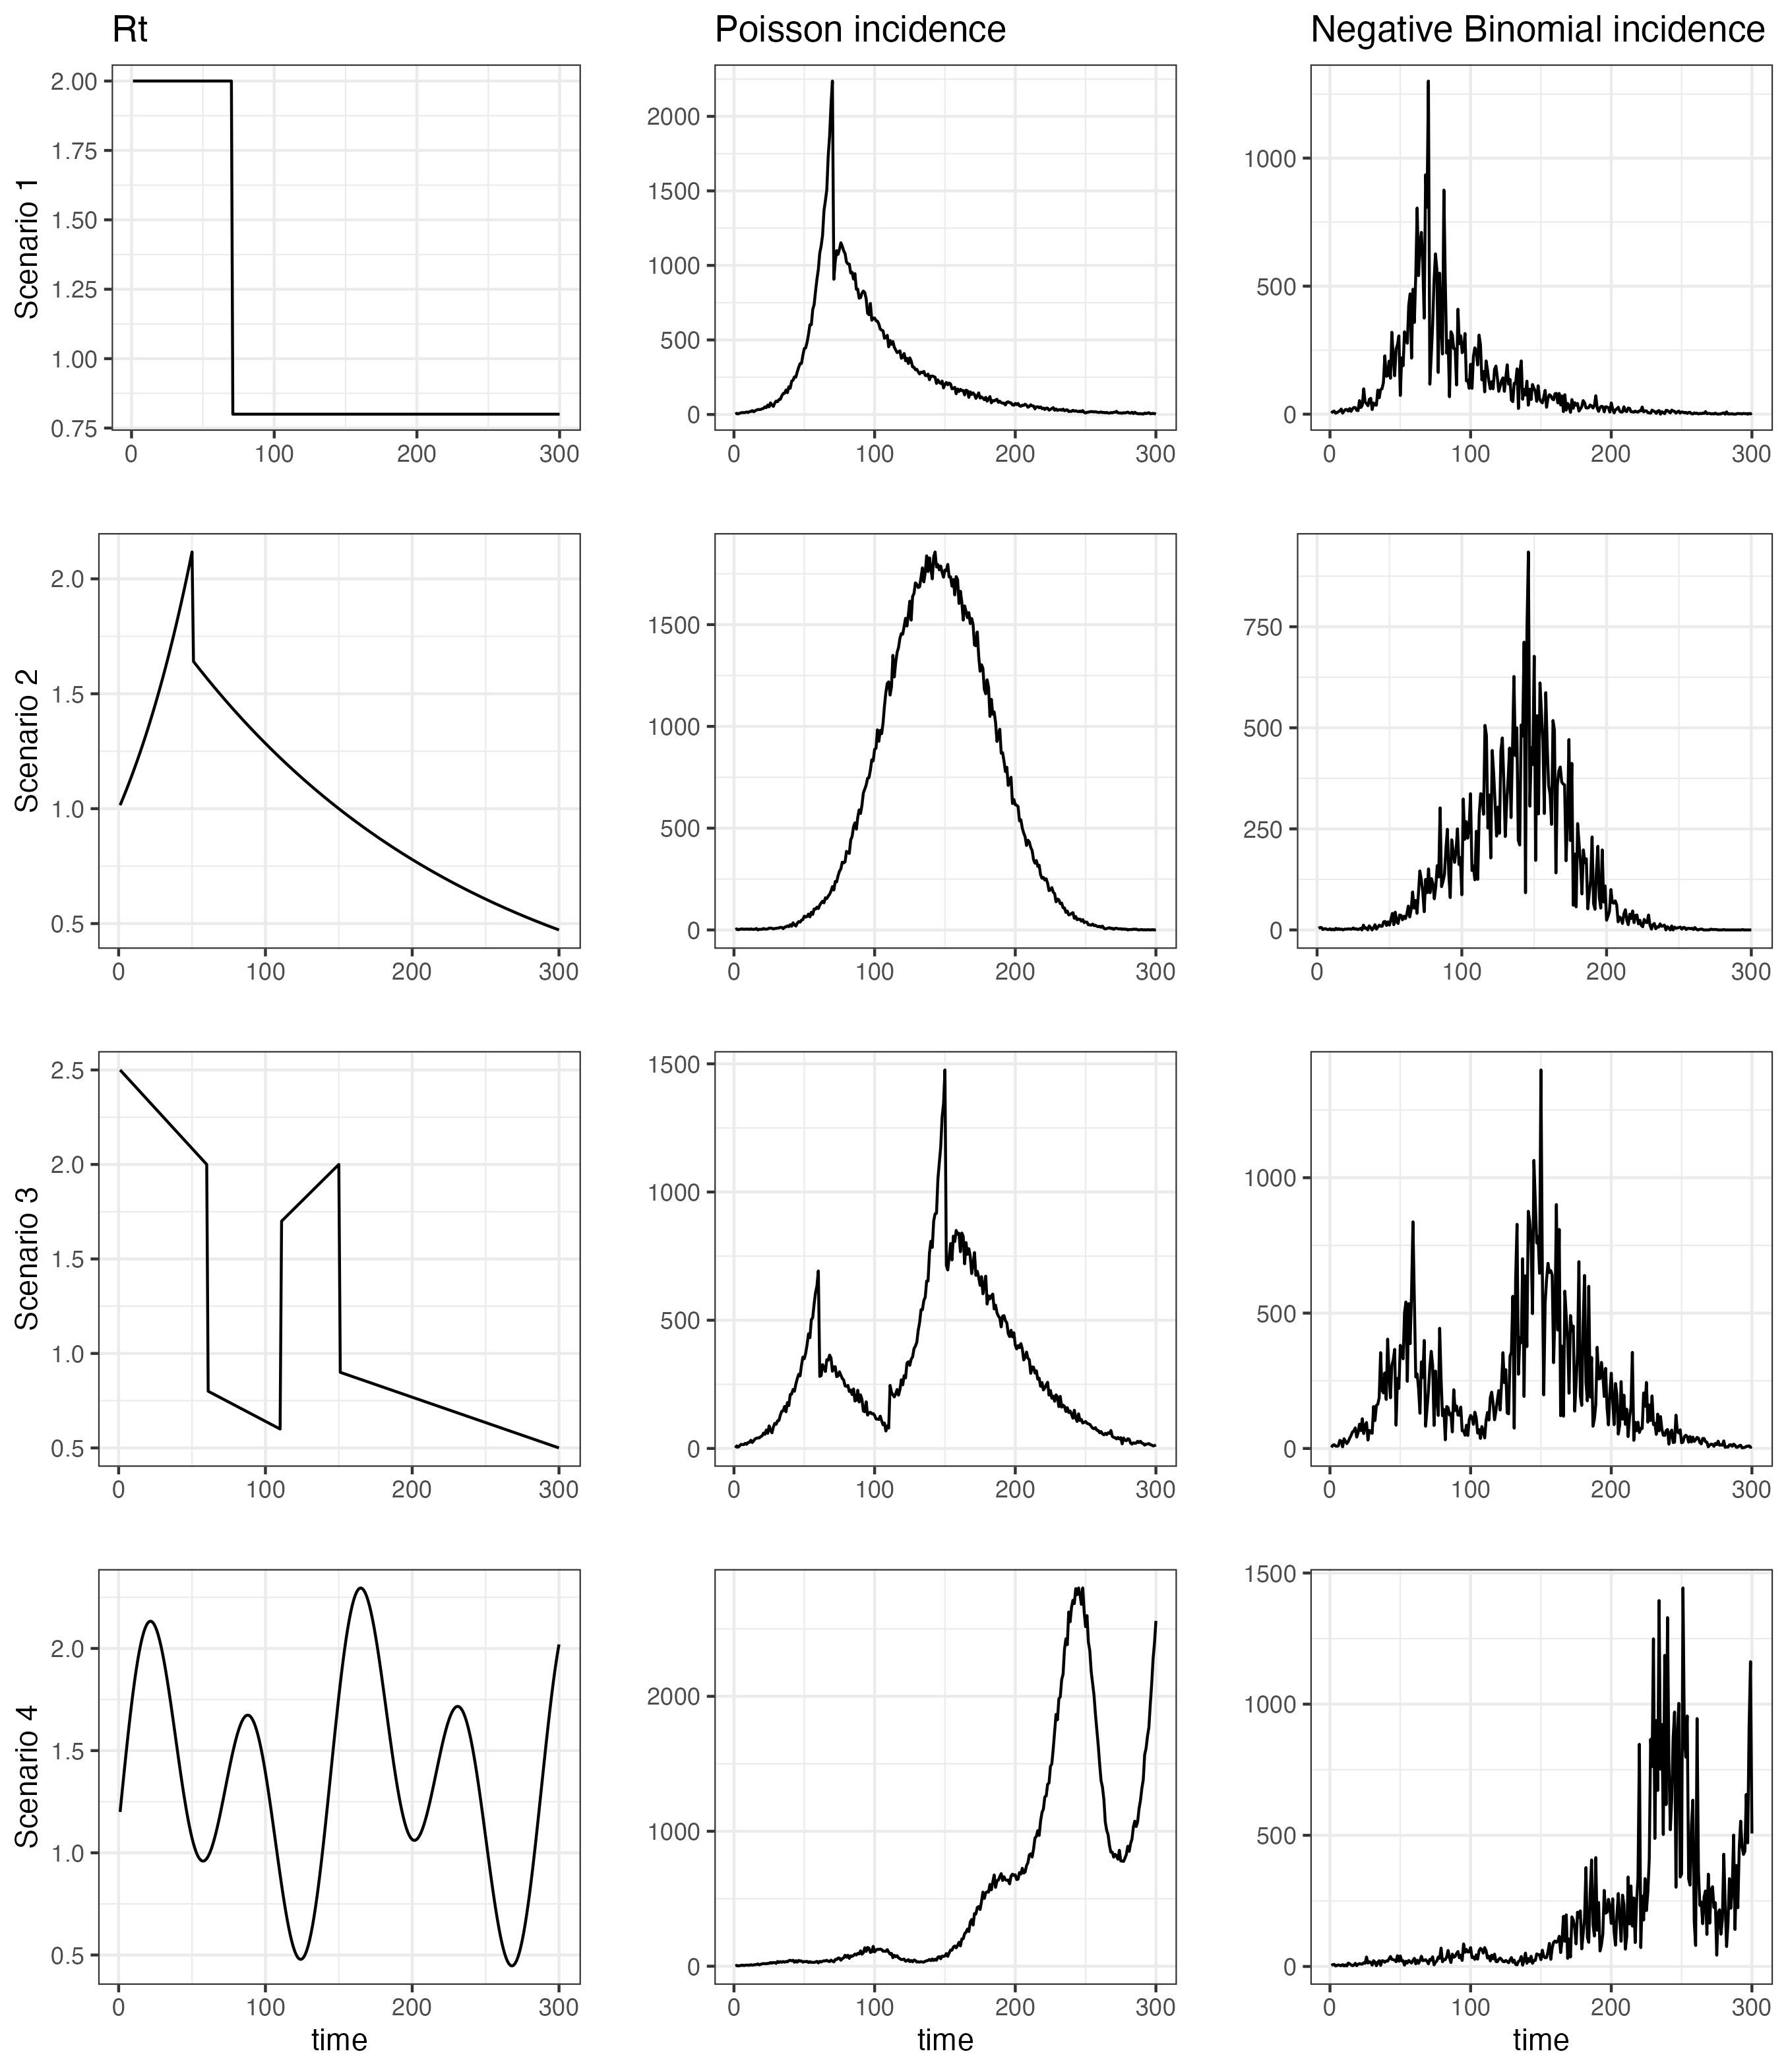
\includegraphics[width=140mm]{fig/plot_samples.png}
    \caption{An example of effective reproduction numbers and corresponding incidences following Poisson or negative Binomial distribution. Three columns illustrate four $\calR_t$ cases, Poisson incidences, and negative Binomial distributed incidences for each $\calR_t$ case respectively. Four rows correspond to four $\calR_t$ cases respectively.} 
    \label{fig:samples}
\end{figure}

% algorithm settings
%% competitors and their settings
We compare our \RtEstim\ to \EpiEstim\ and \EpiLPS. \EpiEstim\ is a widely used Bayesian method that estimates the posterior distribution of effective reproduction numbers given the Gamma prior and Poisson distributed incidences. They estimate the reproduction number over a sliding window by assuming the reproduction number is constant during the specific time window. A longer sliding window averages out more fluctuations and noises, and leads to smoother estimation over time; whereas, a shorter sliding window is more responsive to sudden spikes or declines in a shorter period. We use the default weekly sliding window for the experimental study. Monthly sliding window is also considered in simulation. Since neither of the two sliding windows considerably outperforms the other across all scenarios, we defer the estimation of monthly sliding window to the supplementary document. 
\EpiLPS\ is another Bayesian approach that estimates P-splines coupled with Laplace approximations of the conditional posterior of the spline vector based on negative Binomial distributed incidences. 
%% our RtEstim
We tune the model over the candidate set of size 50 using cross validation. For four scenarios, we estimate piecewise constant $k=0$, piecewise cubic $k=3$, piecewise linear $k=1$ and piecewise cubic polynomials respectively. 
% for all models
We assume the serial intervals are known and use same serial intervals across all models for each problem. 

% KL for exponential family: 
The accuracy of $\calR_t$ estimates is measured by the mean Kullback-Leibler (KL) divergence for Poisson distributions  $$\frac{1}{n} D_{KL}(\hat{\calR}|| \calR) = \frac{1}{n}\sum_{t=1}^n \hat{\calR}_t \log\left(\frac{\hat{\calR}_t}{\calR_t}\right) + {\calR}_t - \hat{\calR}_t,$$ 
where $\calR := \left\{ \calR_t \right\}_{t=1}^n$. %It coincides with the Bregman distance $D_{KL}(\theta_0 || \theta_1) = \varphi(\theta_1) - \varphi(\theta_0) - (\theta_1 - \theta_0)^{\top} \varphi'(\theta_0)$, where $\theta_0,\theta_1$ are natural parameters of the same kind of exponential-family distributions \citep{sadhanala2022exponential}. 
In comparison of the accuracy across methods, we drop the estimates during the first week as the $\calR_t$ estimates of \EpiEstim\ starts at $t=8$. We avoid using the Euclidean ($\ell_2$) norm in favor of KL divergence because Poisson distribution corresponds to points on a discrete lattice, which can be regarded as lying on a curved (non-Euclidean) space in the context of geometry. 
%For negative Binomial cases, we use KL divergence to measure the distances between negative Binomial distributions given the %dispersion rate $\phi$, i.e., 
%\begin{align*}
%    \frac{1}{n} D^{\ast}_{KL}\lr{\hat{\calR}|| \calR} = \frac{1}{n}\sum_{t=1}^n \hat{\calR}_t \log \left(\frac{\hat{\calR}_t}%{\calR_t}\right) + \lr{\hat{\calR}_t + \phi} \log\lr{\frac{\hat{\calR}_t + \phi}{\calR_t + \phi}}. 
%\end{align*}
Other details of the experimental settings are deferred to the supplementary document. 

%\subsubsection*{Cross Validation}
We run leave-third-out cross validation (CV) to choose the best tuning parameter from the candidate set of size $50$, i.e., $\boldsymbol{\lambda} = \{\lambda_1, \cdots, \lambda_{50}\}$. Specifically, we divide the all samples into three folds and build models on each sample set which excludes one fold of the samples across all hyperparameters. Every third samples are placed into the same fold by excluding the first and last samples. We select the tuning parameter that gives the lowest averaged mean squared errors (MSEs) of the estimated reproduction numbers from the observed samples across all folds. 
The experiments are run in \texttt{R} with version 4.3.1 on a MacBook with an Apple M1 Pro chip and RAM 32GB running under macOS Sonoma 14.0. The \texttt{R} packages are of versions \texttt{EpiEstim\_2.2-4}, \texttt{EpiLPS\_1.2.0} and \texttt{rtestim\_0.0.3}. 

\subsection{Experimental results}

% experiment results
\autoref{fig:pois-est} illustrates the estimated reproduction numbers by three models for the Poisson incidence cases. Compared to \EpiEstim\ and \EpiLPS, which have an edge problem at the beginning of the time series, our \RtEstim\ estimates are more accurate --- almost overlap with the true values --- without suffering from the edge problem. Scenario 2 is a difficult problem for all methods; the immediate drop from the end of the exponential growth to the start of the exponential decay is hard to capture for all models. Since we fit a cubic Poisson trend filtering problem for Scenario 2, our estimated $\hat{\calR}_t$ curve is continuous at the knot, which hinders the estimates from fitting the steep decline. 
Scenario 1 is the simplest case with only one knot and two constant segments. Besides the edge problem, \EpiEstim\ and \EpiLPS\ produce ``smooth'' estimated curves that are continuous at the knot, which results in divergence from the true values in the first segment in Scenario 1. Since the piecewise constant \RtEstim\ estimator does not require the smoothness in $\calR_t$, it captures the sharp decrease in Scenario 1. 
\begin{figure}[tb]
    \centering
    \includegraphics*[width=160mm]{fig/Pois-res-plot.png}
    \caption{Effective reproduction number estimation for Poisson incidences.}
    \label{fig:pois-est}
\end{figure}


% experiment results under the violation of assumptions
Under the violation of distributional assumption of incidences, we estimate $\calR_t$s using negative Binomial incidences. \autoref{fig:nb-est} displays the estimates across all methods. \RtEstim\ estimates overall do not perform as remarkably accurate as in the Poisson incidence cases. Especially for Scenario 4, \RtEstim\ fails to recover the wiggly curvature during the first few waves. In Scenario 2, \RtEstim\ succeeds to capture the knot, but suffers from the same problem as in the Poisson cases. In Scenario 3, piecewise linear \RtEstim\ estimates fail to capture the knots and do not fit well during the first half of the time period. 
\begin{figure}[tb]
    \centering
    \includegraphics*[width=160mm]{fig/NB-res-plot.png}
    \caption{Effective reproduction number estimation for negative Binomial incidences.} 
    \label{fig:nb-est}
\end{figure}

\RtEstim\ overall outperforms \EpiEstim\ and \EpiLPS in the experimental study. \autoref{fig:kl-res} visualizes the KL divergences across three models in boxplots. In Scenario 2, the KL divergence boxes of \EpiLPS\ is slightly lower than \RtEstim's boxes, but \EpiLPS\ has large outliers for both Poisson and negative Binomial incidences cases. In general, given the Poisson incidences, \RtEstim\ is more accurate than \EpiEstim\ and \EpiLPS\ across Scenarios 1, 3, 4, and slightly less accurate but more stable than \EpiLPS\ in Scenario 2. Given negative Binomial incidences, \RtEstim\ is still the most accurate in Scenarios 1 and 3, and achieves similar levels of accuracy as \EpiLPS\ (which is based on the negative Binomial distributional assumption on the incidences) in Scenarios 2 and 4. \RtEstim\ has larger outliers than \EpiLPS\ for Scenarios 1, 3, and 4 given negative Binomial incidences, but the difference is no more than $0.1$. 
\begin{figure}[htb]
    \centering
    \includegraphics*[width=160mm]{fig/kl.png}
    \caption{Boxplot of Kullback-Leibler divergence between the estimated effective reproduction numbers and the true ones across all methods given Poisson incidences and negative Binomial incidences across 50 samples. Left panel visualizes the KL divergences for the Poisson incidence cases. Right panel displays the KL divergences for the negative Binomial incidence cases. Outliers (larger than $3$) of EpiEstim is excluded for a better visualization.} 
    \label{fig:kl-res}
\end{figure}

We also compare the running times of three models across $8$ experimental settings. We find that all models across all experiments takes less than $3$ seconds to converge. Our model runs longer generally, which is likely due to a relatively large candidate set (of size $50$), other models only run a single time for a fixed set of hyperparameters per experiment. 
More experimental results on time comparisons are deferred to the supplementary document. 


\subsection{Covid-19 incidences in British Columbia}

% introduce data & tuning parameter setup
We implement our \RtEstim\ on the Covid-19 confirmed cases in British Columbia (B.C.) as of May 18, 2023 (visualized in \autoref{fig:covid-data}) reported by B.C. Centre for Disease Control. We choose the gamma distribution with shape $2.5$ and scale $2.5$ to approximate the serial interval function, which is empirically found to be a reasonable choice. 
\begin{figure}[tb]
    \centering
    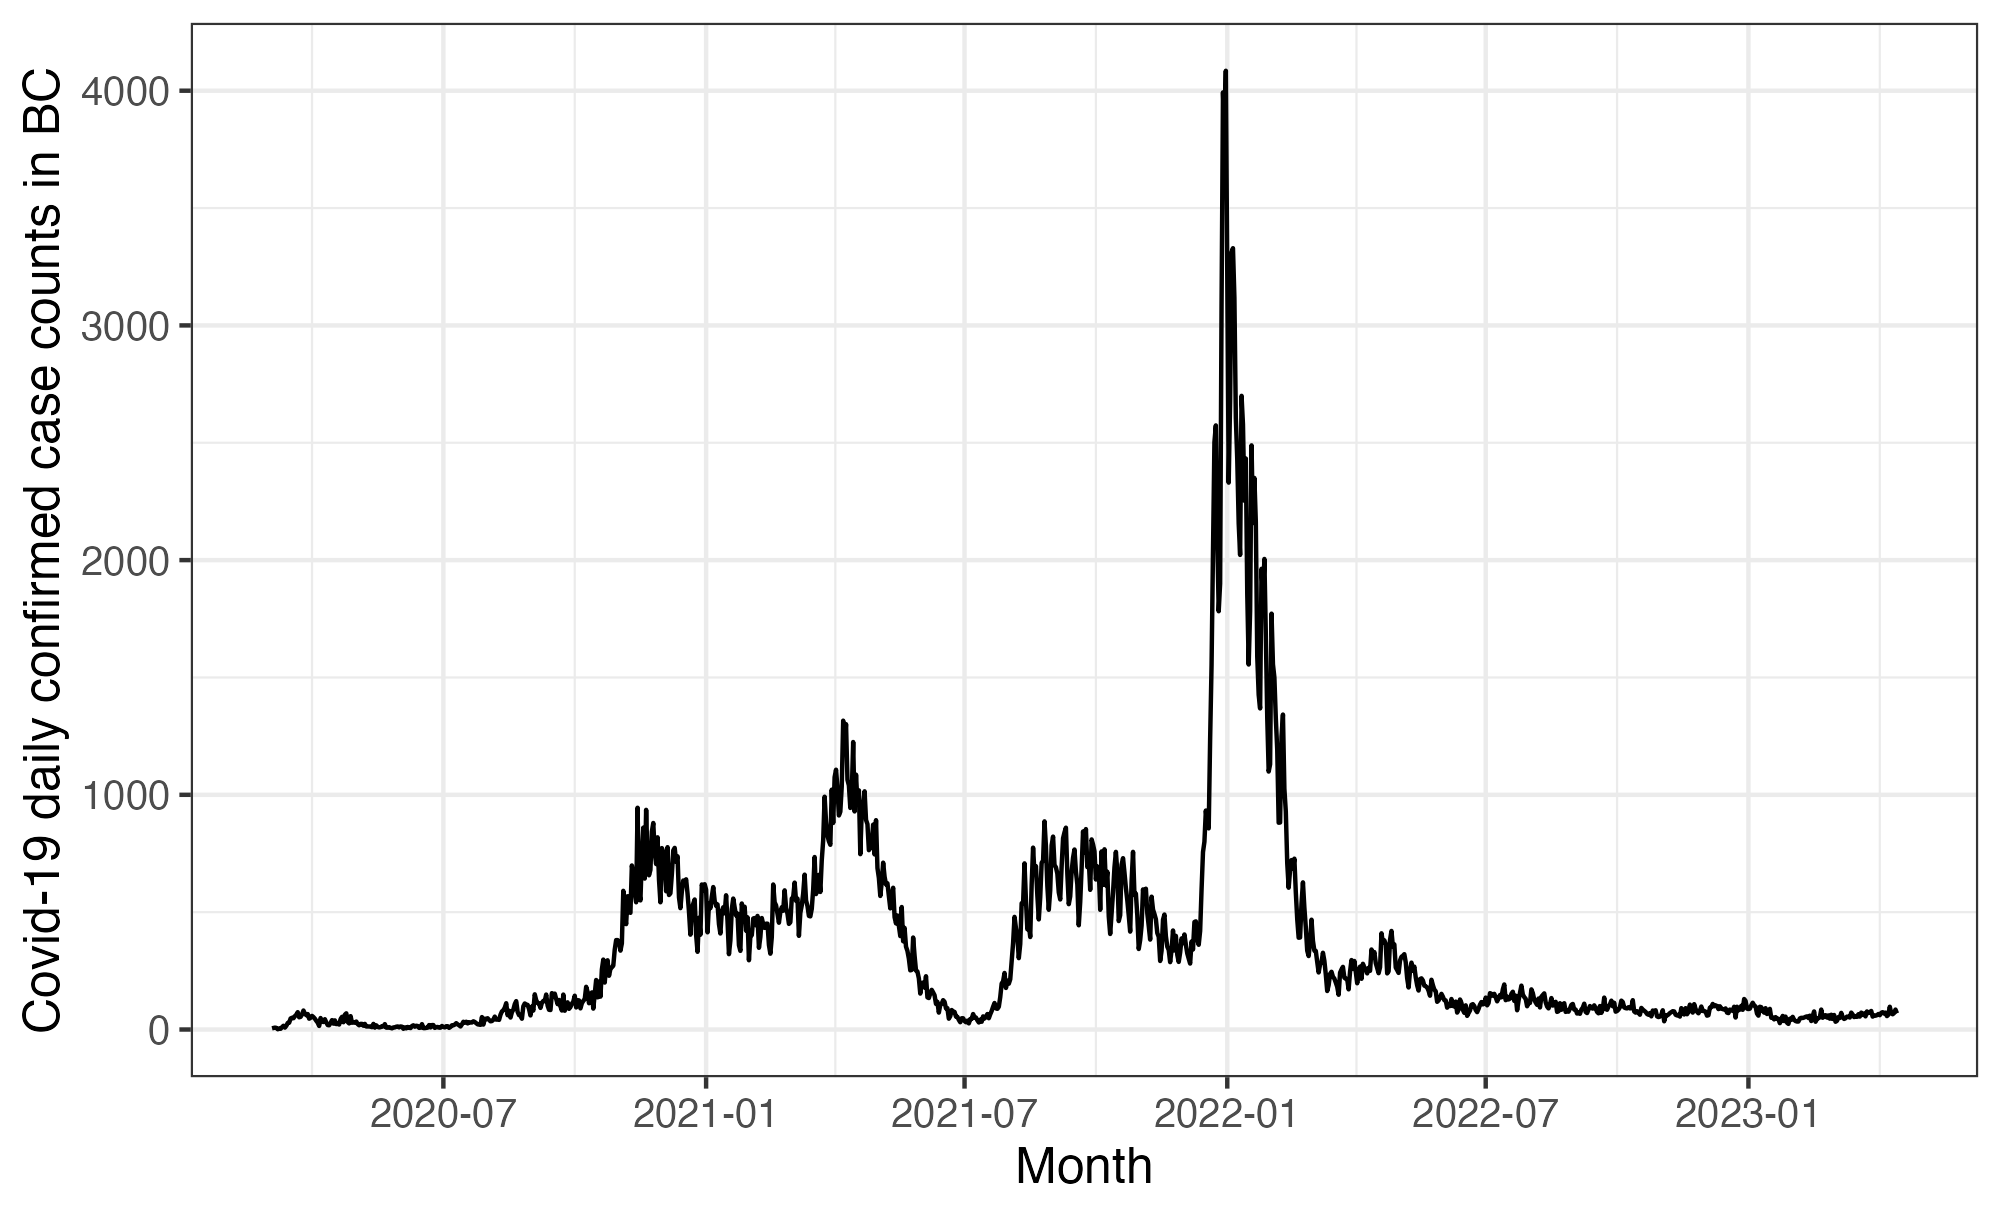
\includegraphics[width=0.99\linewidth]{fig/covid_dat.png}
    \caption{Covid19 daily confirmed incidence counts between March 1st, 2020 and April 15th, 2023 in British Columbia, Canada.} 
    \label{fig:covid-data}
\end{figure} 

% interpret figures -- across all lambdas
Considering the temporal evolutions of effective reproduction numbers across $3, 4, 5$ days, the estimated reproduction numbers of Covid-19 in British Columbia (illustrated in \autoref{fig:covid-rt}) are less than $3$ during most of the time, which means that one distinct infected individuals can on average infect less than three other individuals in the population. The three degrees of the temporal evolution (across all regularization levels $\lambda$) all yield similar results that $\hat{\calR}_t$ comes to the highest peak around the end of 2021 and then drops down to the lowest trough shortly thereafter. Throughout the estimated curves, the peaks and troughs of the reproduction numbers roughly come prior to the following growths and decays of confirmed cases respectively.
% CBs for real epidemic applications
We also visualize the 95\% empirical confidence bands of the point estimates for the ``best'' tuning parameter (in terms of MSEs). 

The reproduction numbers are relatively unstable before April 1st, 2022. The highest peak coincides with the emergence and globally spread of the Omicron variant. The estimated reproduction numbers are apparently below the threshold $1$ during two time periods -- roughly from April 1st, 2021 to July 1st, 2021 and from January 1st, 2022 to April 1st, 2022. The first trough coincides with the first authorization for use of Covid-19 vaccines in British Columbia. The second trough shortly after the greatest peak may credit to many aspects, including self-isolation of the infected individuals and application of the second shot of Covid-19 vaccines. Since around April 1st, 2022, the reproduction numbers stay stable (fluctuating around $1$) and the infected cases stay low. 

% for different lambda
Greater regularization levels (by using larger $\lambda$s) result in smoother estimated curves. Smoother curves suggest that the estimated reproduction numbers are around $1$ during most time periods; however, it may miss to capture some outbreaks of the pandemic. More wiggly curves better reflect the fluctuation of $\calR_t$, but sometimes fail to highlight the significant peaks or troughs. The tuning parameter $\lambda$ needs to be chosen corresponding to the information in practice for a better interpretation. Here, we provide the CV-chosen $\calR_t$ estimates with confidence bands. 
\begin{figure}[tb]
    \centering
    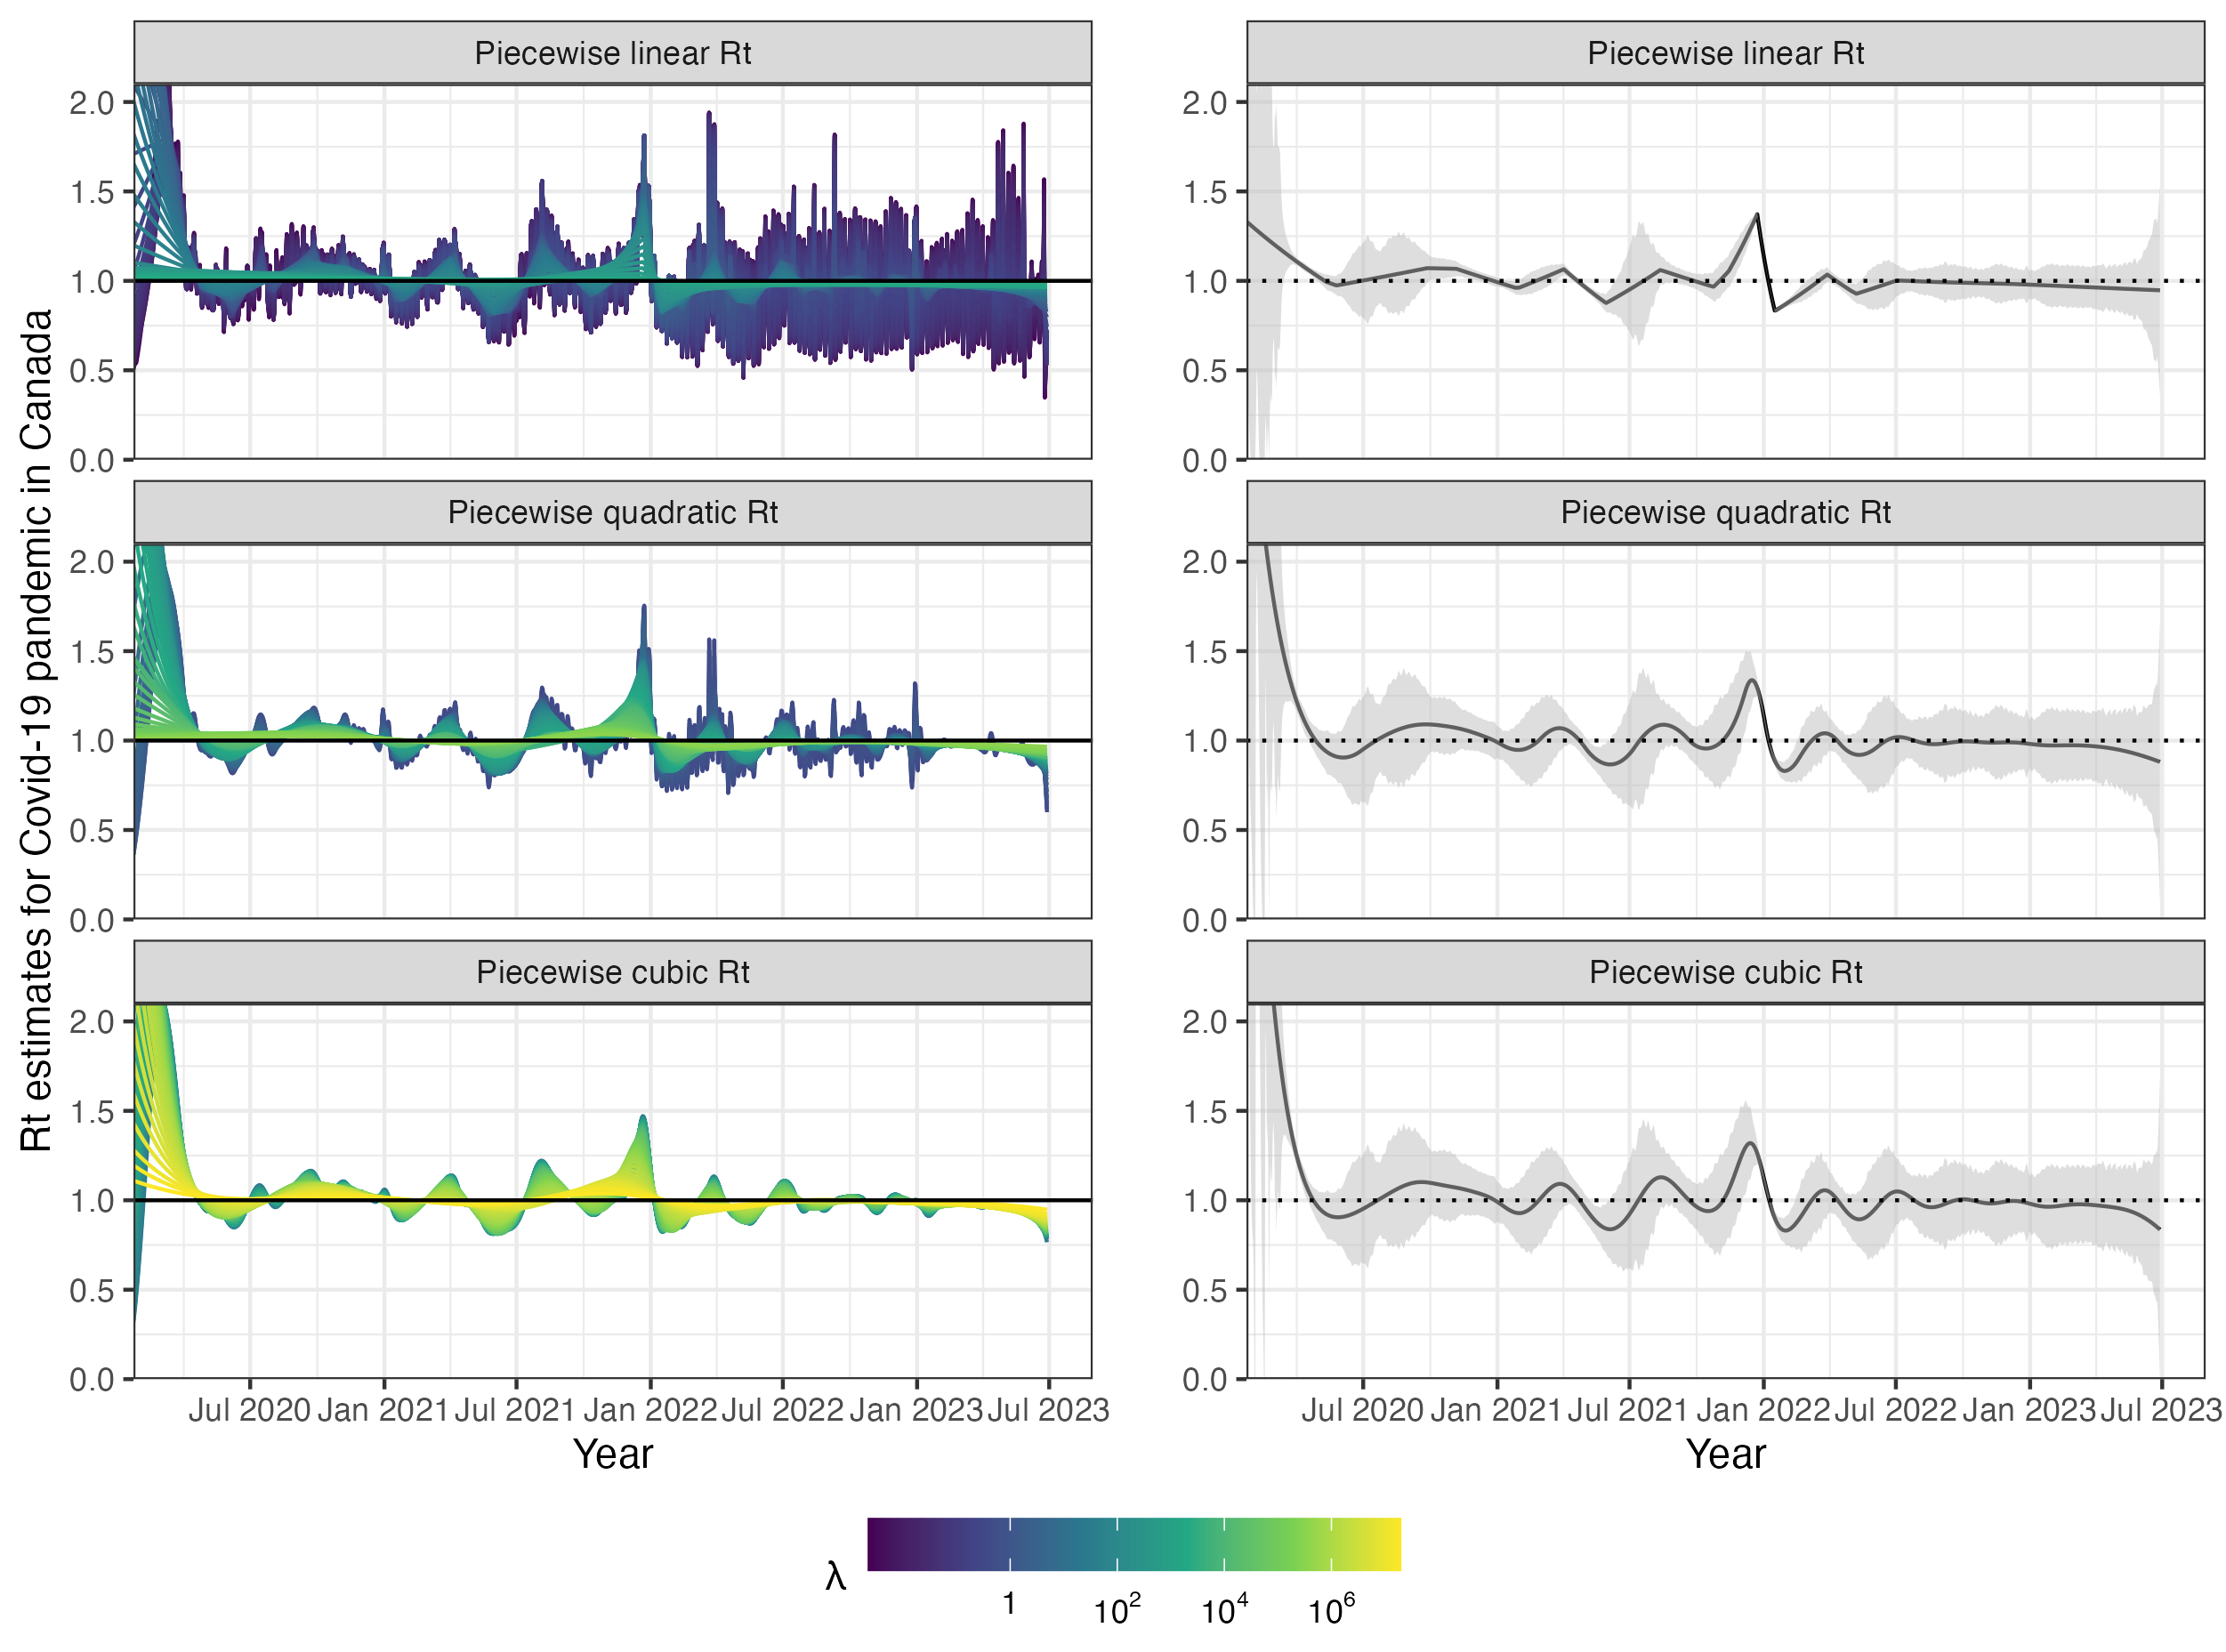
\includegraphics[width=0.99\linewidth]{fig/covid_full_res.png}
    \caption{Estimated effective reproduction numbers for Covid19 daily confirmed counts between March 1st, 2020 and April 15th, 2023 in British Columbia, Canada. The left panels display the CV-tuned estimates with 95\% confidence intervals. The right panels demonstrate estimates corresponding to 50 tuning parameters. The top, medium and bottom panels illustrate the estimated reproduction numbers ($\calR_t$) using the Poisson trend filtering (in \eqref{eq:rt-ptf}) with degrees $k=1,2,3$ respectively.} 
    \label{fig:covid-rt}
\end{figure} 


\subsection{Pandemic influenza in Baltimore, Maryland, 1918}

We then apply \RtEstim\ on the pandemic influenza in Baltimore, Maryland, 1918. Dataset in \autoref{fig:flu-dat} is obtained from the \texttt{R} package \EpiEstim. The 1918 influenza, caused by H1N1 influenza A virus, was an unprecedentedly deadly influenza that infected almost one-third of the population across the world \citep{taubenberger20061918}. 
In the estimation displayed in \autoref{fig:flu-res}, the CV-tuned piecewise cubic estimates better capture the growing tendency at the beginning of the pandemic. It suggests that the pandemic has yielded a decrease after around 20 days and reached $1$ when the pandemic has lasted for nearly 50 days. However, it also suggests an increase at the end of the period, while a steady decline (as in CV-tuned piecewise constant and linear estimates) is more reasonable. The smoothness of $\calR_t$ curves should be chosen based on the purpose of the study in practice, e.g., epidemic forecasting may require a more wiggly curve that contains more fluctuation information, while retrospective studies that solely target on understanding of the pandemic may prefer a smoother curve with less important information smoothed out. 
\begin{figure}[tb]
    \centering
    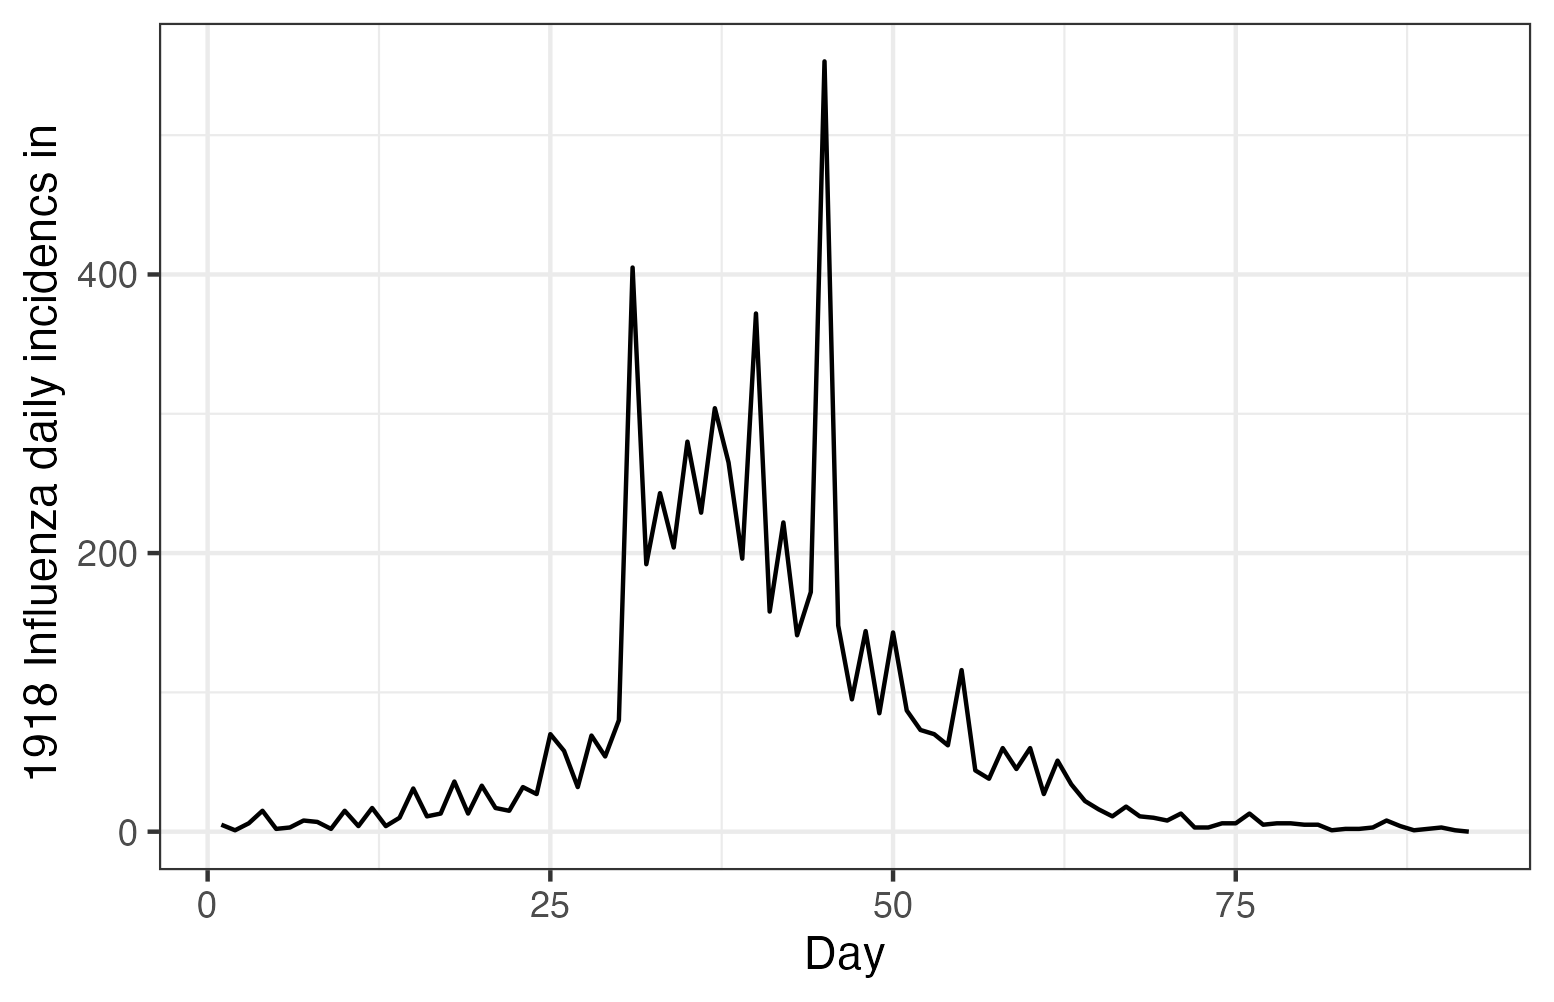
\includegraphics[width=0.9\linewidth]{fig/flu_dat.png}
    \caption{Pandemic influenza incidence counts in Baltimore, Maryland in 1918.} 
    \label{fig:flu-dat}
\end{figure} 

\begin{figure}[tb]
    \centering
    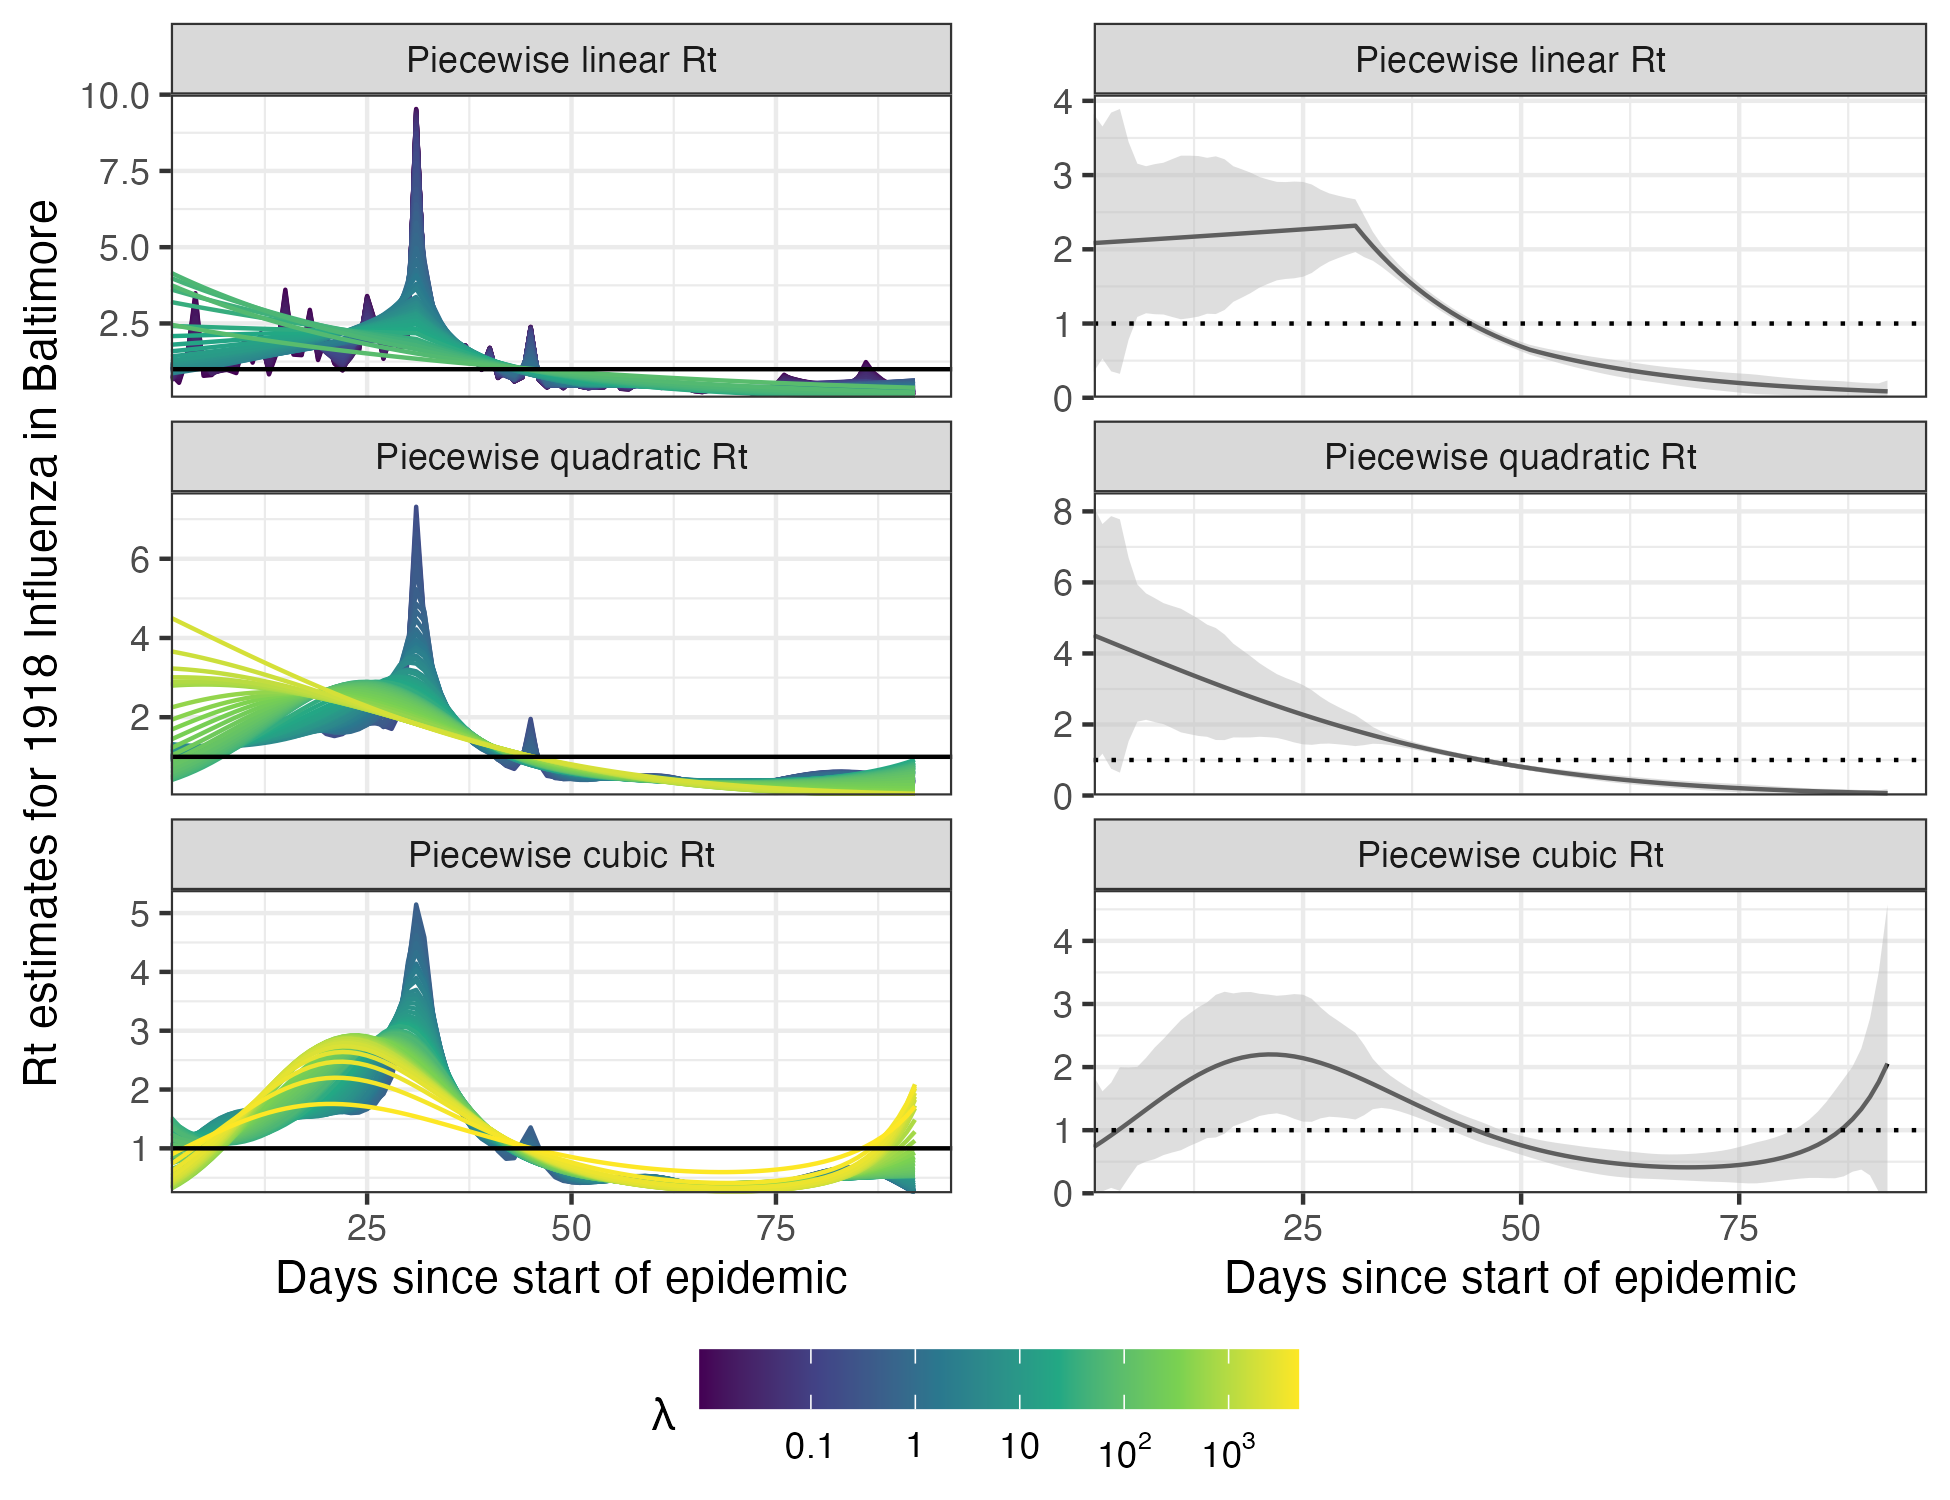
\includegraphics[width=0.9\linewidth]{fig/flu_full_res.png}
    \caption{Estimated effective reproduction numbers for pandemic influenza incidence counts in Baltimore, Maryland in 1918. The left panels display the CV-tuned estimates with 95\% confidence intervals. The right panels demonstrate estimates corresponding to 50 tuning parameters. The top, medium and bottom panels illustrate the estimated reproduction numbers ($\calR_t$) using the Poisson trend filtering (in \eqref{eq:rt-ptf}) with degrees $k=1,2,3$ respectively.} 
    \label{fig:flu-res}
\end{figure} 


\section{Discussion}

The \RtEstim\ methodology provides a locally adaptive estimator using Poisson
trend filtering on univariate data. It captures the heterogeneous smoothness of
effective reproduction numbers given observed incidence data rather than
resulting in global smoothness. This is a nonparametric regression model which
can be written as a convex optimization (minimization) problem. Minimizing the
distance (KL divergence across all coordinates) between the estimators and
(functions of) observations guarantees data fidelity while the penalty on divided
differences between pairs of neighbouring parameters imposes smoothness. The
$\ell_1$-regularization results in sparsity of the divided differences, which
leads to heterogeneous smoothness across time. 


The property of local adaptivity (heterogenous smoothness) is useful to
automatically distinguish, for example, seasonal outbreaks from outbreaks driven
by other factors (behavioural changes, foreign introduction, etc.). Given a
well-chosen polynomial degree, the growth rates can be quickly detected, 
potentially advising public health to implement policy changes. The effective
reproduction numbers can be estimated retrospectively to examine the efficacy of
such policies, whether they result in $\calR_t$ falling below 1 or the speed of
their effects. The smoothness of $\calR_t$ curves (including the polynomial 
degrees and tuning parameters) should be chosen based on the purpose of the 
study in practice, e.g., epidemic forecasting may require less smoothness
while retrospective studies that 
solely target understanding of the pandemic may prefer a smoother estimate. 


Our method \RtEstim\ provides a natural way to deal with missing data, for
example, on weekends and holidays or due to changes in reporting frequency.
While solving the convex optimization problem, our method can easily 
handle uneven spacing or irregular reporting. Computing the total
primary infectiousness is also easily generalized to irregular reporting by
modifying the discretization of the serial interval distribution. Additionally,
because the $\ell_1$ penalty introduces sparsity (operating like a median
rather than a mean), this procedure is relatively insensitive to outliers
compared to $\ell_2$ regularization.


There are a number of limitations that may influence the quality of
$\calR_t$ estimation. While our model is generic for incidence data 
rather than tailored to any specific disease, it does assume that the 
generation interval is short relative to the period of data collection. 
More specialized methodologies would be required for diseases with long 
incubation periods such as HIV or Hepatitis. 
Our approach, does not explicitly model imported cases, nor distinguish between
subpopulations that may have different mixing behaviour. 
While the Poisson assumption is common, it does not handle overdispersion
(observation variance larger than the mean). The negative binomial distribution
is a good alternative, but more difficult to estimate in this context.
As described in \autoref{sec:intro}, the expression for $\calR$ 
assumes that a relatively constant proportion of true infections is reported. 
However, if this proportion varies with time (say, due to changes in surveillance
practices or testing recommendations), the estimates may be biased over this
window. A good example is in early January 2022, during the height of the
Omicron wave, British Columbia moved from testing all symptomatic individuals to
testing only those in at-risk groups. The result was a sudden change that would
render $\calR_t$ estimates on either side of this timepoint incommensurable.


As currently implemented, \RtEstim\ uses a fixed serial interval throughout the
period of study, but as factors such as population immunity vary, the serial
interval may vary as well \citep{nash2023estimating}.  
Another issue relates to equating serial and generation intervals (also
mentioned above). The serial interval distribution is generally wider than that
of the generation interval, because the serial interval involves the convolution
of two distributions, and is unlikely to actually follow a named distribution
like Gamma, though it may be reasonably well approximated by one. Our
implementation allows for an arbitrary distribution to be used, but requires the
user to specify the discretization explicitly, requiring more nuanced knowledge
than is typically available. Pushing this analysis further, to accommodate other
types of incidence data (hospitalizations or deaths), a modified generation
interval distribution would be necessary, and further assumptions would be
required as well. Or else, one would first need to deconvolve deaths to
infection onset before using our software.


Nonetheless, our methodology is implemented in a lightweight \R\ package 
\texttt{rtestim} and computed efficiently, especially for large-scale data, 
with a proximal Newton solver coded in \cpp. 
Given available incident case data, prespecified serial interval
distribution, and a choice of degree $k$, \RtEstim\ is able to produce
accurate estimates of effective reproduction number and provide efficient
tuning parameter selection via cross validation. 


%\section*{Acknowledgement}


\addcontentsline{toc}{section}{References}
\bibliography{doc/ptf}

%\appendix
%\titleformat{\chapter}{\normalfont\huge\bfseries}{Appendix \thechapter}{1em}{}

\end{document}
